\documentclass[11pt,a4paper]{article}
\usepackage[utf8]{inputenc}
\usepackage[margin=1in]{geometry}
\usepackage{amsmath,amssymb}
\usepackage{booktabs}
\usepackage{graphicx}
\usepackage{hyperref}
\usepackage{xcolor}
\usepackage{microtype}
\usepackage{subcaption}
\usepackage{float}
\usepackage{fancyhdr}

\hypersetup{
    colorlinks=true,
    linkcolor=blue!75!black,
    citecolor=blue!75!black,
    urlcolor=blue!75!black
}

\pagestyle{fancy}
\fancyhf{}
\rhead{\small Workshop No. 1 — Data Preparation \& Baselines}
\lhead{\small Machine Learning (2026-III) — Gr. 1}
\rfoot{\small Page \thepage}

\title{\LARGE \textbf{Workshop No. 1: Data Preparation \& Supervised Learning Baselines}\\
\large Real Estate Valuation Benchmark on the Ames Housing Dataset}

\author{
    \textbf{Group 1} \\
    Chavez Porras Miguel Alejandro (ID: 20212020033) \\
    Guerrero Ordeñez Luisa Fernanda (ID: 20212020099) \\
    Arboleda Zambrano Dilan Stive (ID: 20212020105) \\
    \vspace{0.25cm} \\
    \textit{Faculty of Engineering, Computer Engineering Program} \\
    \textit{Universidad Distrital Francisco José de Caldas} \\
    \textit{Professor: Eng. Carlos Andrés Sierra, M.Sc.}
}

\date{October 26, 2026}

\begin{document}

\maketitle

\begin{abstract}
This report presents the complete data engineering, exploratory analysis, and supervised baseline modeling for Workshop No. 1 in the Machine Learning course. Utilizing the authoritative Ames Housing dataset ($N = 2,930$ residential records, 82 features) compiled by Dean De Cock (2011), we build a strictly leak-free preprocessing pipeline and benchmark three classic machine learning regression paradigms: Regularized Linear Regression (Ridge), an ensemble of randomized decision trees (Random Forest Regressor), and Gradient Boosting Regressor (GBR). We characterize the severe positive skewness ($+1.744$) and heteroscedasticity of raw residential sale prices, demonstrate variance stabilization via the log-transform $\log(1 + y)$, resolve structural categorical absences versus genuine missing values, and isolate high-leverage outliers. Under a strictly held-out $70\%/15\%/15\%$ train/validation/test split saved to \texttt{data/splits.json}, our best baseline model—Gradient Boosting—achieves a Mean Absolute Error (MAE) of \$14,876.80, a Test $R^2$ of $0.8672$, and a Root Mean Squared Logarithmic Error (RMSLE) of $0.1208$. All code, splits, figures, and models are fully reproducible through standard command line scripts.
\end{abstract}

\section{Executive Summary}
Accurate real estate valuation is a quintessential tabular machine learning problem governed by heterogeneous attribute types, non-linear physical interactions, and spatial clustering. 

The principal conclusions of this workshop are summarized as follows:
\begin{enumerate}
    \item \textbf{Target Distributional Geometry:} The raw dependent variable \texttt{SalePrice} is markedly right-skewed ($\text{skew} = +1.744$, $\text{kurtosis} = 5.119$). Training linear or tree models directly on raw dollar figures causes excessive penalization of luxury homes and heteroscedastic residuals. Transforming the target via $y^* = \log(1 + y)$ contracts right-tail dispersion, producing near-symmetric residuals ($\text{skew} = -0.061$, $\text{kurtosis} = 1.218$) and significantly enhancing generalization stability.
    \item \textbf{Structural Absence vs. Missingness:} Real estate datasets feature apparent ``missing'' values that represent physical absence rather than uncollected data (e.g., $99.6\%$ missing in \texttt{Pool QC}, $93.2\%$ in \texttt{Alley}, and $48.5\%$ in \texttt{Fireplace Qu}). Converting these instances to explicit categorical levels (\texttt{'None'}) and imputing corresponding numerical spaces with zeros preserves vital predictive information.
    \item \textbf{Outlier Diagnostics and Training Cleansing:} Dean De Cock (2011) identified five properties exceeding 4,000 square feet of living area, where three represented atypical agricultural or partial-interest transfers priced far below market value. Pruning these anomalous observations strictly from the training partition prevents distorted regression hyperplanes without compromising out-of-sample evaluation integrity.
    \item \textbf{Strict Leakage Prevention Protocol:} Imputation values (including neighborhood-conditional lot frontages), feature scalers (RobustScaler), and target transformation parameters were computed exclusively on the $70\%$ training partition and projected onto the validation and test partitions without recomputation.
    \item \textbf{Empirical Baseline Hierarchy:} Gradient Boosting achieved the superior test error balance ($\text{MAE} = \$14,876.80$, $\text{RMSLE} = 0.1208$, $R^2 = 0.8672$), followed by Ridge Regression ($\text{MAE} = \$15,031.51$, $\text{RMSLE} = 0.1254$) and Random Forest ($\text{MAE} = \$16,700.76$, $\text{RMSLE} = 0.1325$). Tree-based models identified \texttt{Overall Qual}, total living area (\texttt{TotalSF}), and year built as the primary determinants of residential value.
\end{enumerate}

\section{Dataset Description and Integrity Verification}

\subsection{Data Origin and Context}
The Ames Housing dataset was curated by Dean De Cock of Truman State University and published in the \textit{Journal of Statistics Education} (Vol. 19, No. 3, 2011). It documents 2,930 residential real estate transactions in Ames, Iowa, occurring between 2006 and 2010. Designed to modernize and replace the heavily flawed 1978 Boston Housing dataset, Ames encompasses 80 domain-specific explanatory features capturing physical footprint, structural materials, architectural quality, basement and garage configurations, and geographic location.

\subsection{Acquisition and Cryptographic Checksums}
The raw dataset and its accompanying assessor documentation were acquired directly from the official publication server. To ensure uncompromising reproducibility across research groups, cryptographic checksums were verified at the moment of download:
\begin{itemize}
    \item \textbf{Primary Host:} Journal of Statistics Education, American Statistical Association
    \item \textbf{Raw Ingestion URL:} \url{http://jse.amstat.org/v19n3/decock/AmesHousing.txt}
    \item \textbf{Assessor Codebook URL:} \url{http://jse.amstat.org/v19n3/decock/DataDocumentation.txt}
    \item \textbf{Raw TSV File Size:} 960,807 bytes
    \item \textbf{Raw TSV MD5:} {\footnotesize \texttt{c2997eb69ab4bf946b9fbdb7e6805e36}}
    \item \textbf{Raw TSV SHA-256:} {\scriptsize \texttt{6cfe6cb525ba437de428653a1040e2aed7d696640bf75203786a6d7a0e67cfcc}}
    \item \textbf{Canonical CSV File Size:} 987,811 bytes
    \item \textbf{Canonical CSV SHA-256:} {\scriptsize \texttt{5d5d25c60c165143749013a89a86c604fd55bac07c2a2e6e0d6c9dacf65e6226}}
\end{itemize}

An automated integrity auditing script was written in \texttt{src/dataset\_info.py}. When executed, it checks local files against these checksums and summarizes dataset dimensions before downstream execution begins.

\subsection{Variable Typology and Summary Statistics}
The raw dataset consists of 82 columns, including an observation order index (\texttt{Order}), the Ames Assessor Parcel Identification Number (\texttt{PID}), and the dependent variable (\texttt{SalePrice}). 

The remaining 80 explanatory variables are distributed across four statistical measurement types:
\begin{itemize}
    \item \textbf{Nominal (23 features):} Unordered categorical descriptors such as \texttt{Neighborhood} (28 distinct districts), \texttt{Bldg Type} (Single-family, Townhouse, Duplex), \texttt{Foundation} (Poured Concrete, Cinder Block, Brick), and \texttt{Sale Condition}.
    \item \textbf{Ordinal (23 features):} Categorical assessments with inherent qualitative ordering, such as \texttt{Overall Qual}, \texttt{Exter Qual}, \texttt{Bsmt Qual}, and \texttt{Kitchen Qual} (evaluated on a standardized scale: Excellent, Good, Typical/Average, Fair, Poor, None).
    \item \textbf{Discrete (14 features):} Countable integer quantities representing house components, including \texttt{Year Built}, \texttt{Year Remod/Add}, \texttt{Full Bath}, \texttt{Bedroom AbvGr}, and \texttt{Fireplaces}.
    \item \textbf{Continuous (20 features):} Spatial and linear dimensions recorded in square or linear feet, including \texttt{Lot Frontage}, \texttt{Lot Area}, \texttt{Total Bsmt SF}, \texttt{1st Flr SF}, \texttt{Gr Liv Area}, and \texttt{Garage Area}.
\end{itemize}

Table~\ref{tab:target_stats} summarizes the central tendencies and dispersion metrics of the target variable in both raw currency and log-transformed space.

\begin{table}[H]
\centering
\caption{Target Variable (\texttt{SalePrice}) Summary Statistics ($N = 2,930$)}
\label{tab:target_stats}
\begin{tabular}{lrr}
\toprule
\textbf{Metric} & \textbf{Raw Sale Price (USD)} & \textbf{Log Transformed $\log(1 + y)$} \\
\midrule
Sample Count       & 2,930               & 2,930           \\
Mean               & \$180,796.06        & 12.022          \\
Median             & \$160,000.00        & 11.983          \\
Standard Deviation & \$79,886.69         & 0.406           \\
Minimum            & \$12,789.00         & 9.456           \\
25th Percentile    & \$129,500.00        & 11.771          \\
75th Percentile    & \$213,500.00        & 12.271          \\
Maximum            & \$755,000.00        & 13.534          \\
Skewness           & \textbf{+1.744}     & \textbf{-0.061} \\
Kurtosis           & \textbf{+5.119}     & \textbf{+1.218} \\
\bottomrule
\end{tabular}
\end{table}

\section{Exploratory Data Analysis (EDA)}
We implemented a dedicated exploratory pipeline in \texttt{src/eda\_generator.py} and encapsulated the complete interactive workflow in \texttt{notebooks/eda.ipynb}.

\subsection{Target Distribution Dynamics}
Figure~\ref{fig:target_dist} contrasts the distribution of \texttt{SalePrice} prior to and following the logarithmic transformation. The raw distribution manifests heavy right-tailed asymmetry caused by luxury homes retailing between \$350,000 and \$755,000. Under logarithmic transformation, the skewness decreases from $+1.744$ to $-0.061$, and kurtosis drops from $5.119$ to $1.218$. This stabilization eliminates heteroscedasticity, satisfying the Gauss-Markov assumptions required for regularized linear estimators.

\begin{figure}[H]
\centering
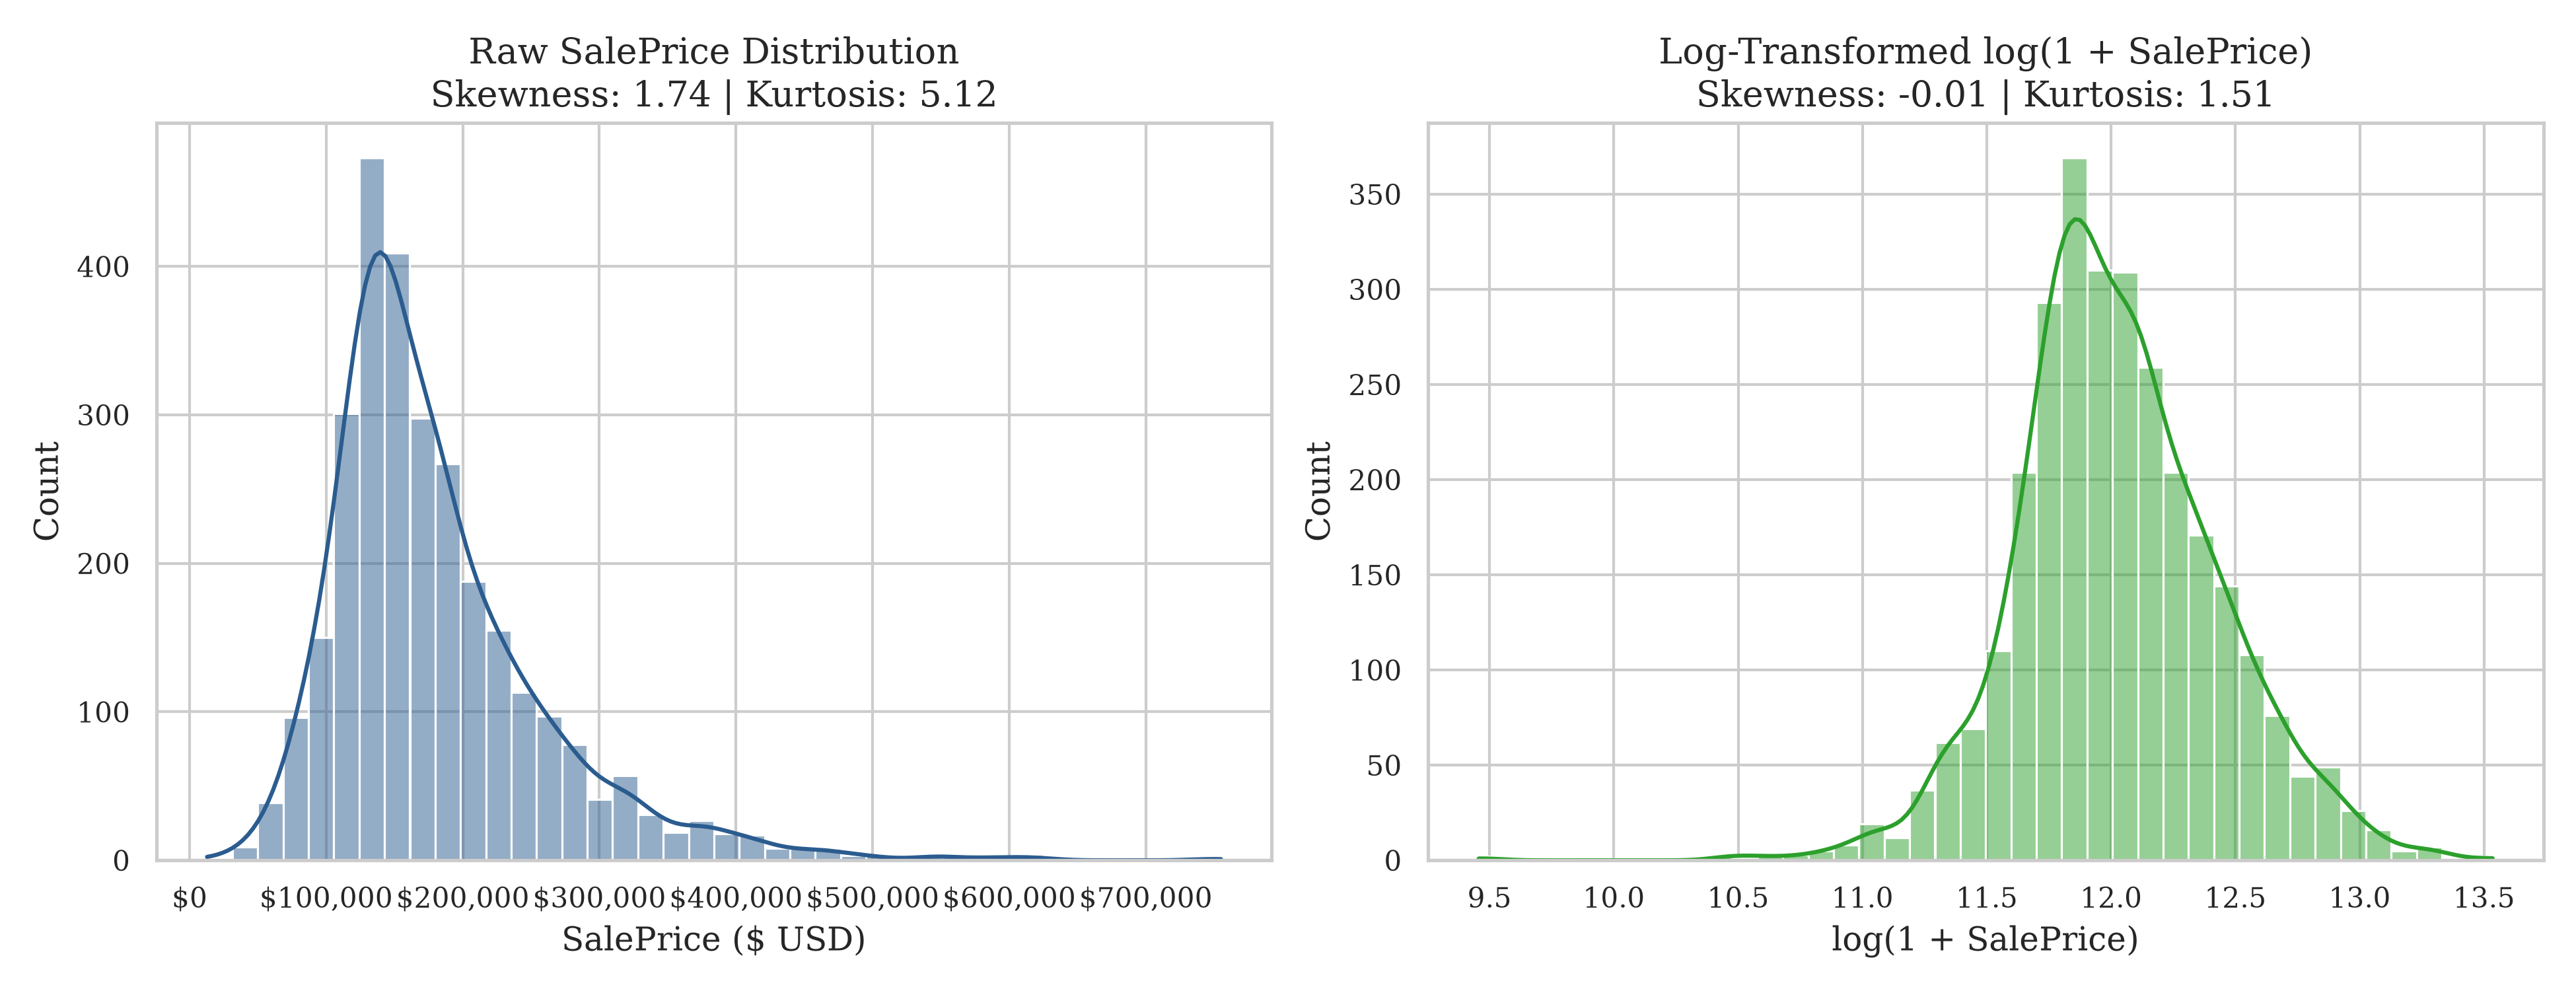
\includegraphics[width=0.92\textwidth]{../results/figures/target_distribution.png}
\caption{Distributional geometry of the dependent variable \texttt{SalePrice}: Raw distribution (left) vs. $\log(1 + \text{SalePrice})$ transformed distribution (right).}
\label{fig:target_dist}
\end{figure}

\subsection{Missingness Mechanisms and Quality Assessment}
Twenty-seven variables contain missing entries. However, as illustrated in Figure~\ref{fig:missing_bar}, the highest proportions occur in features associated with optional property structures: \texttt{Pool QC} (99.6\%), \texttt{Misc Feature} (96.4\%), \texttt{Alley} (93.2\%), \texttt{Fence} (80.5\%), and \texttt{Fireplace Qu} (48.5\%). In real estate valuation, an unrecorded pool or fireplace indicates that the property does not possess that amenity, rather than a failure of record-keeping. Dropping these rows would discard over 99\% of the observations; conversely, imputing them with the statistical mode would falsely ascribe luxury amenities to typical residences. They are consequently retained as explicit informative absent categories.

\begin{figure}[H]
\centering
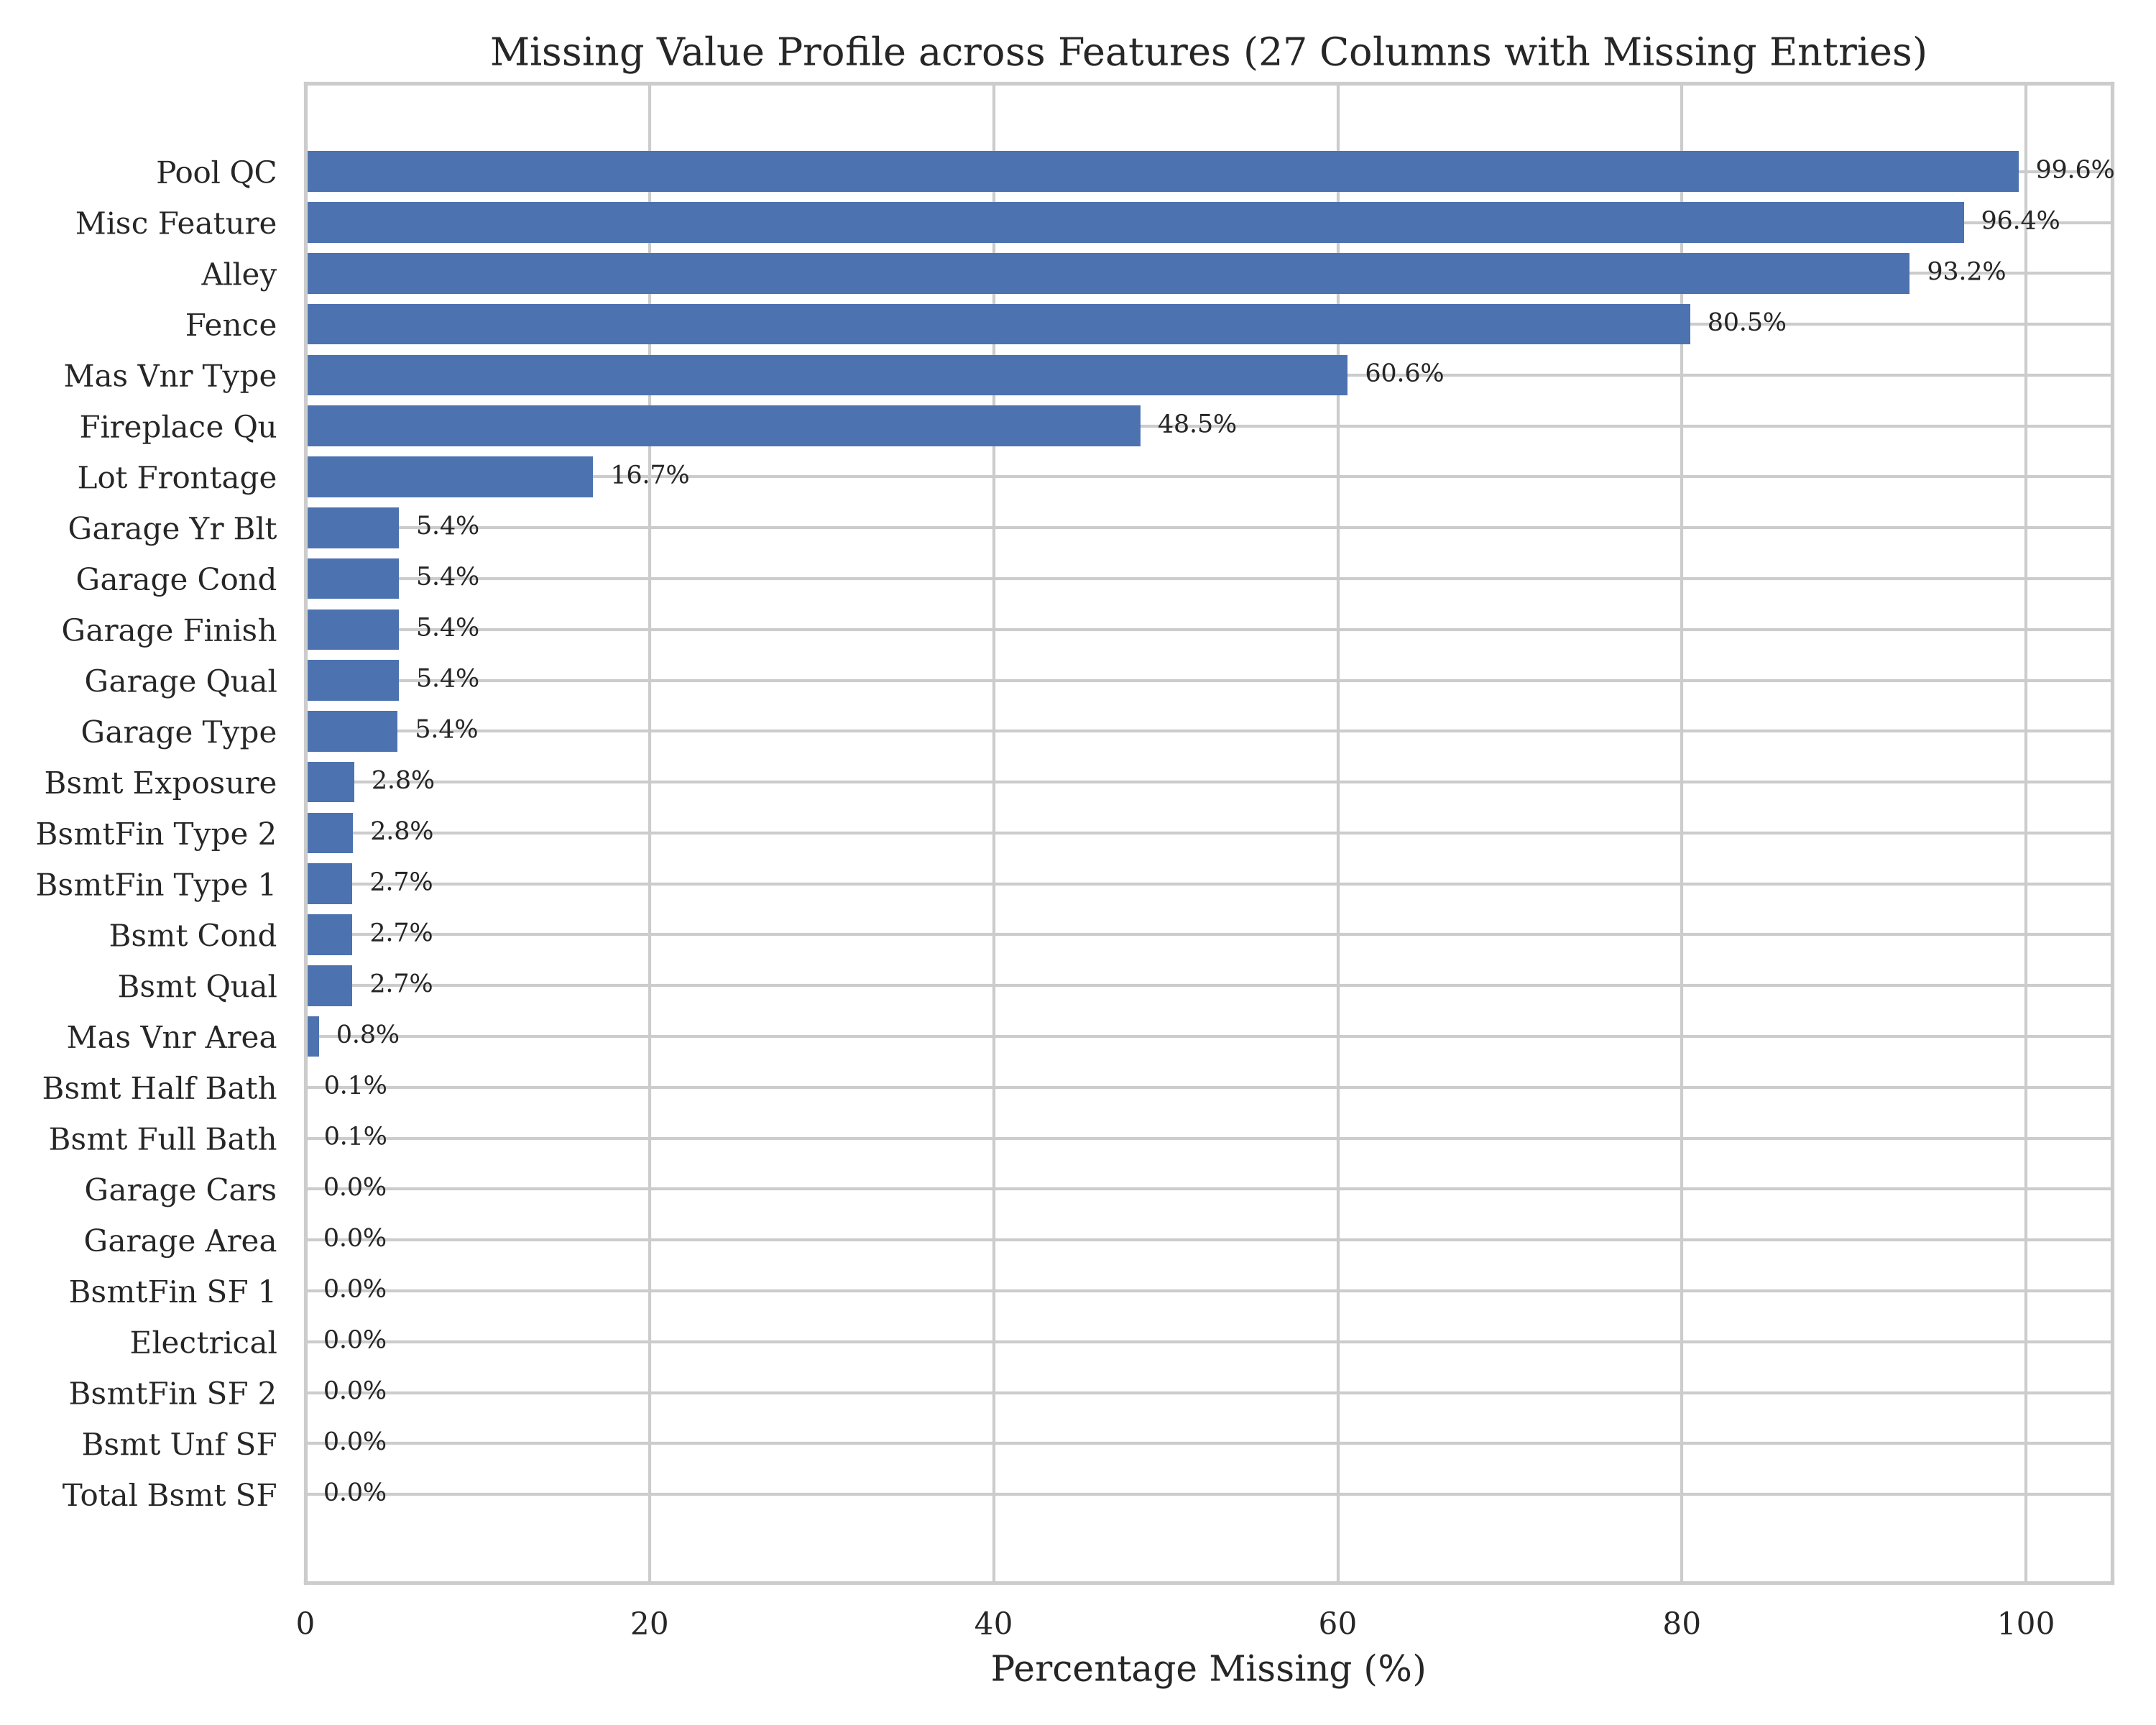
\includegraphics[width=0.82\textwidth]{../results/figures/missing_values_bar.png}
\caption{Percentage of missing entries across all affected features in the Ames Housing dataset.}
\label{fig:missing_bar}
\end{figure}

For continuous variables such as \texttt{Lot Frontage} (16.7\% missing), missingness correlates with subdivision plotting practices. Because lot widths are geographically determined by local zoning codes, we compute the median frontage on a per-neighborhood basis exclusively on the training partition.

\subsection{Identification of Influential Outliers}
Dean De Cock (2011) explicitly cautioned against retaining atypical transactions exceeding 4,000 square feet of above-ground living area. Figure~\ref{fig:outliers} inspects the relationship between \texttt{Gr Liv Area} and \texttt{SalePrice}. Two properties (PID \texttt{0528151010} with 5,642 sq ft and PID \texttt{0528166100} with 4,676 sq ft) were sold for \$160,000 and \$184,750 respectively under partial-interest sales conditions. These observations exhibit extreme leverage, distorting the slope of ordinary least squares estimators. We remove these two anomalous records exclusively during training fitting.

\begin{figure}[H]
\centering
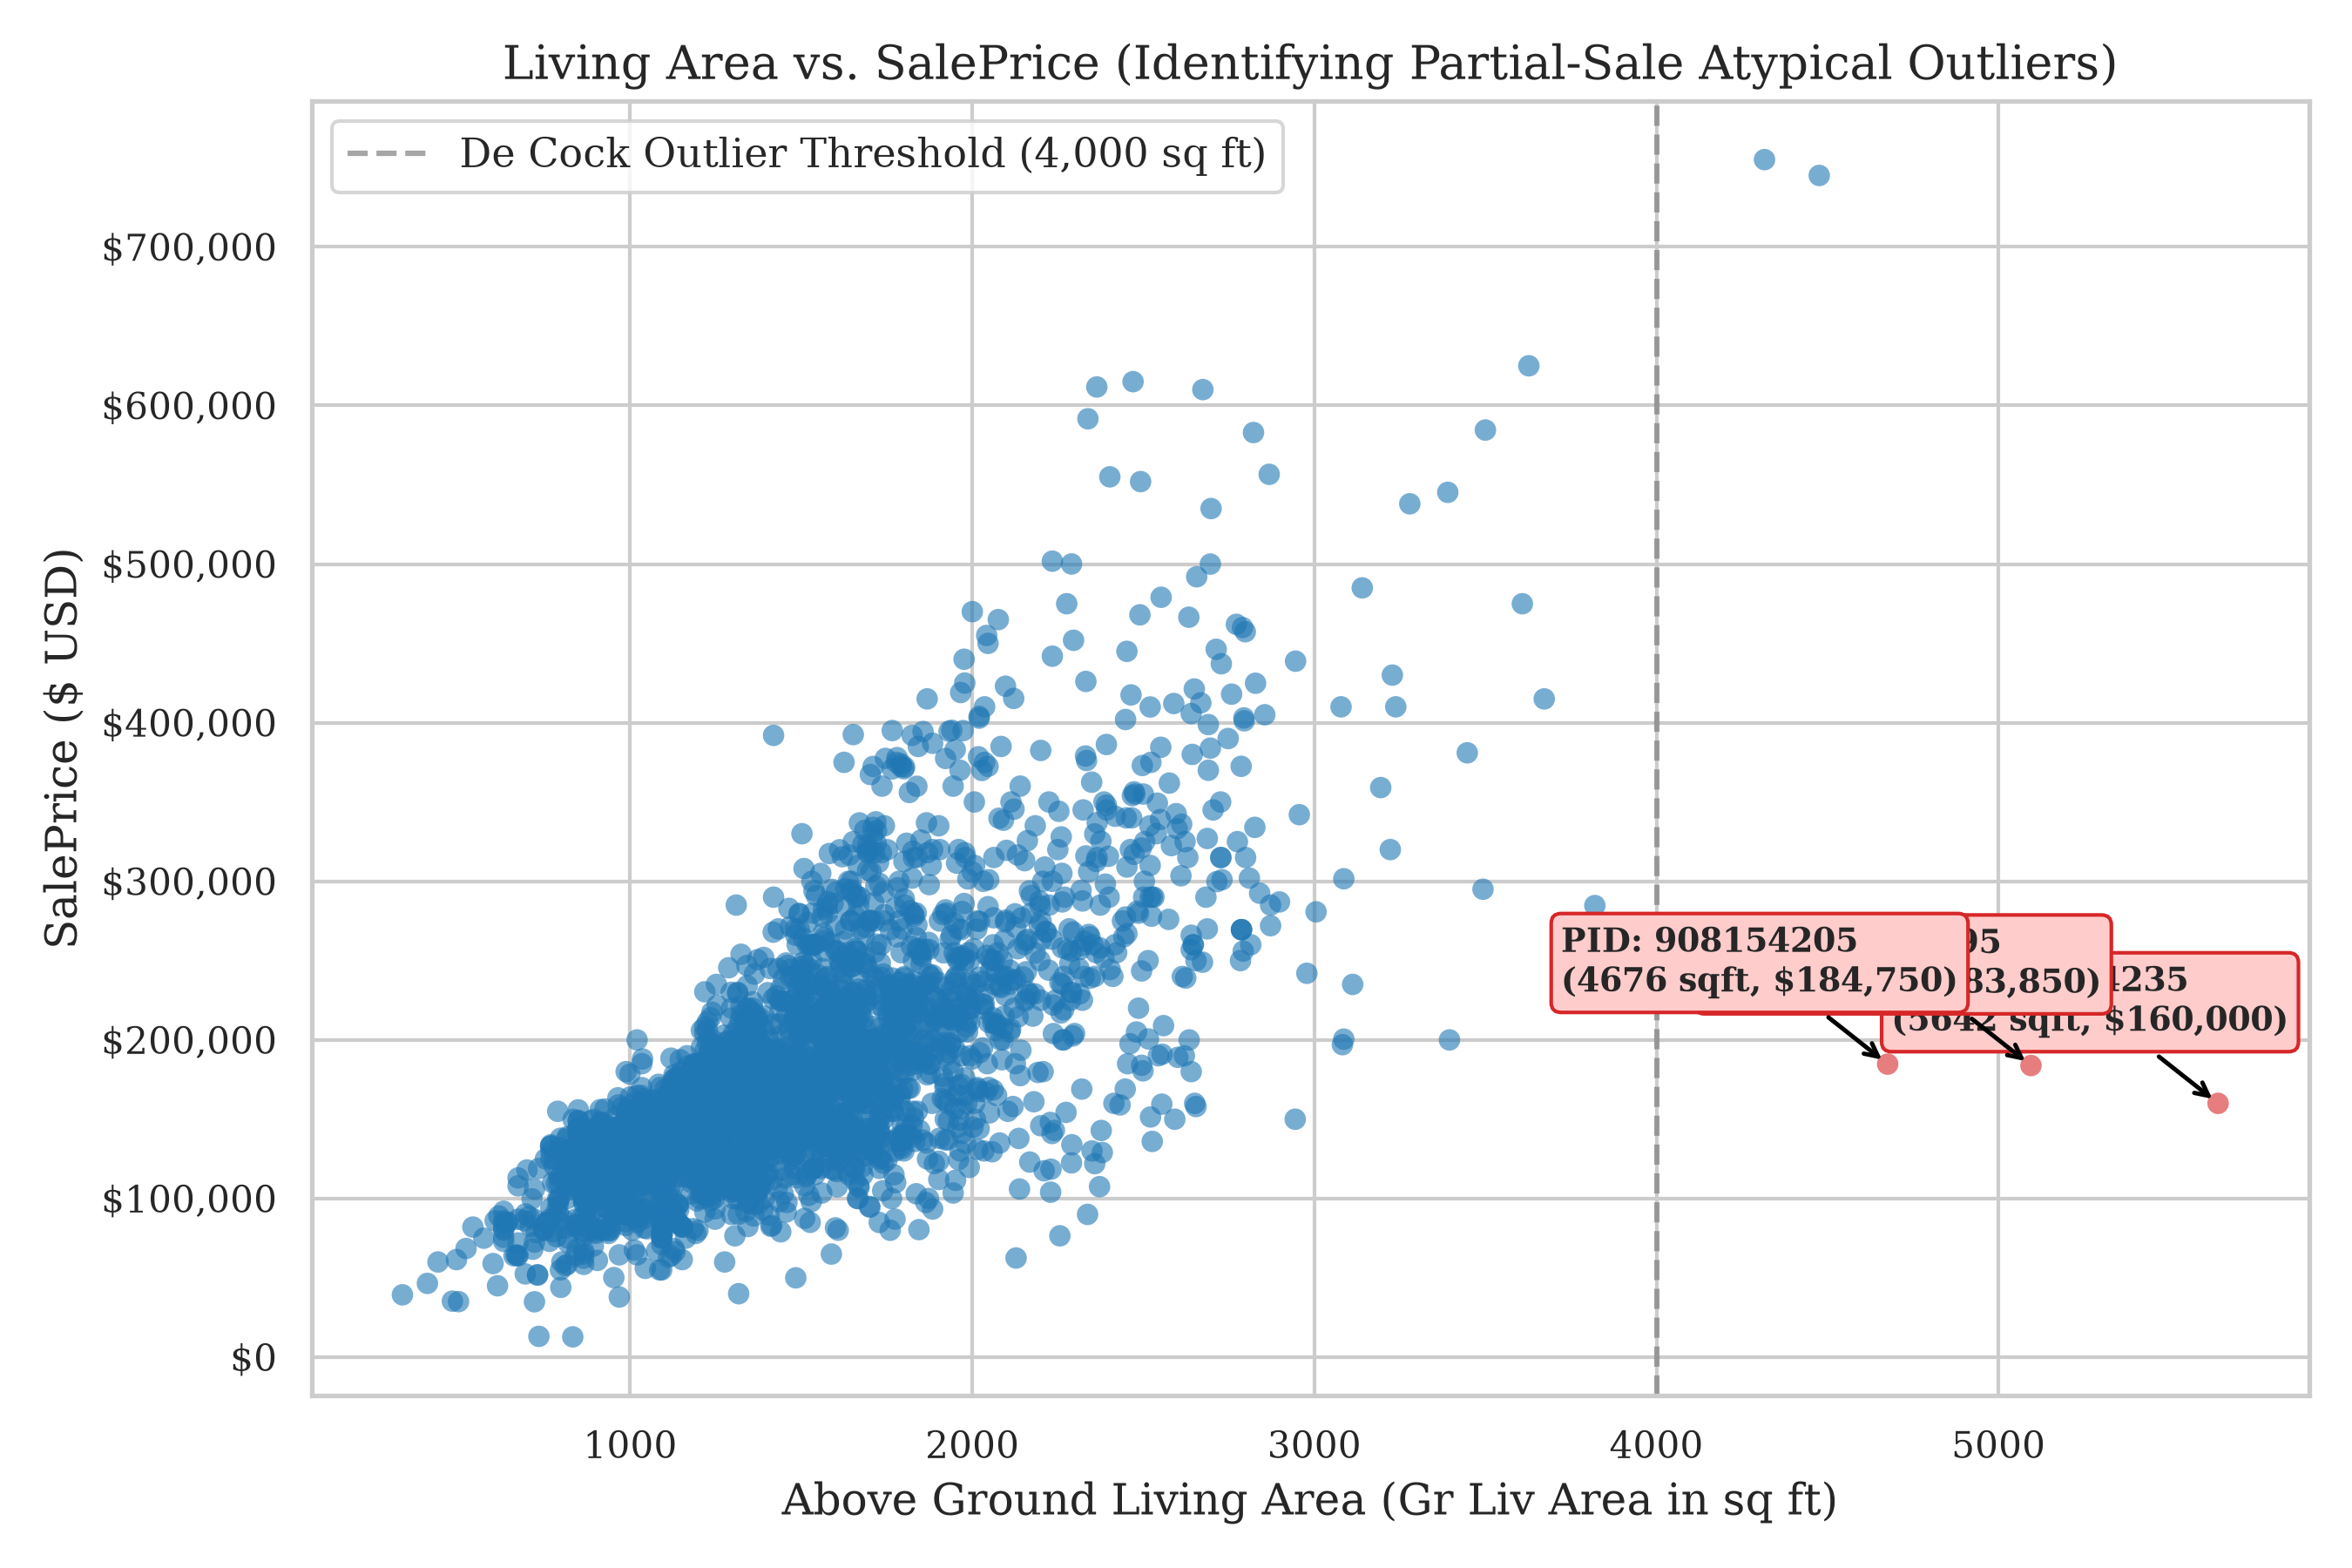
\includegraphics[width=0.72\textwidth]{../results/figures/outliers_grlivarea.png}
\caption{Scatter plot of Above-Ground Living Area vs. SalePrice, isolating the high-leverage outliers ($> 4,000$ sq ft, $<\$300,000$).}
\label{fig:outliers}
\end{figure}

\subsection{Feature Correlation Structure and Valuation Drivers}
Figure~\ref{fig:correlation} presents the correlation matrix among the numerical features most strongly associated with home prices. \texttt{Overall Qual} demonstrates the strongest linear correlation ($r = 0.80$), followed by \texttt{Gr Liv Area} ($r = 0.71$), \texttt{Total Bsmt SF} ($r = 0.63$), \texttt{Garage Cars} ($r = 0.65$), and \texttt{Year Built} ($r = 0.56$). Furthermore, collinearity is observed between size metrics (\texttt{1st Flr SF} and \texttt{Total Bsmt SF}, $r = 0.80$; \texttt{Garage Cars} and \texttt{Garage Area}, $r = 0.89$), highlighting the necessity of $L_2$ regularization in linear baselines.

\begin{figure}[H]
\centering
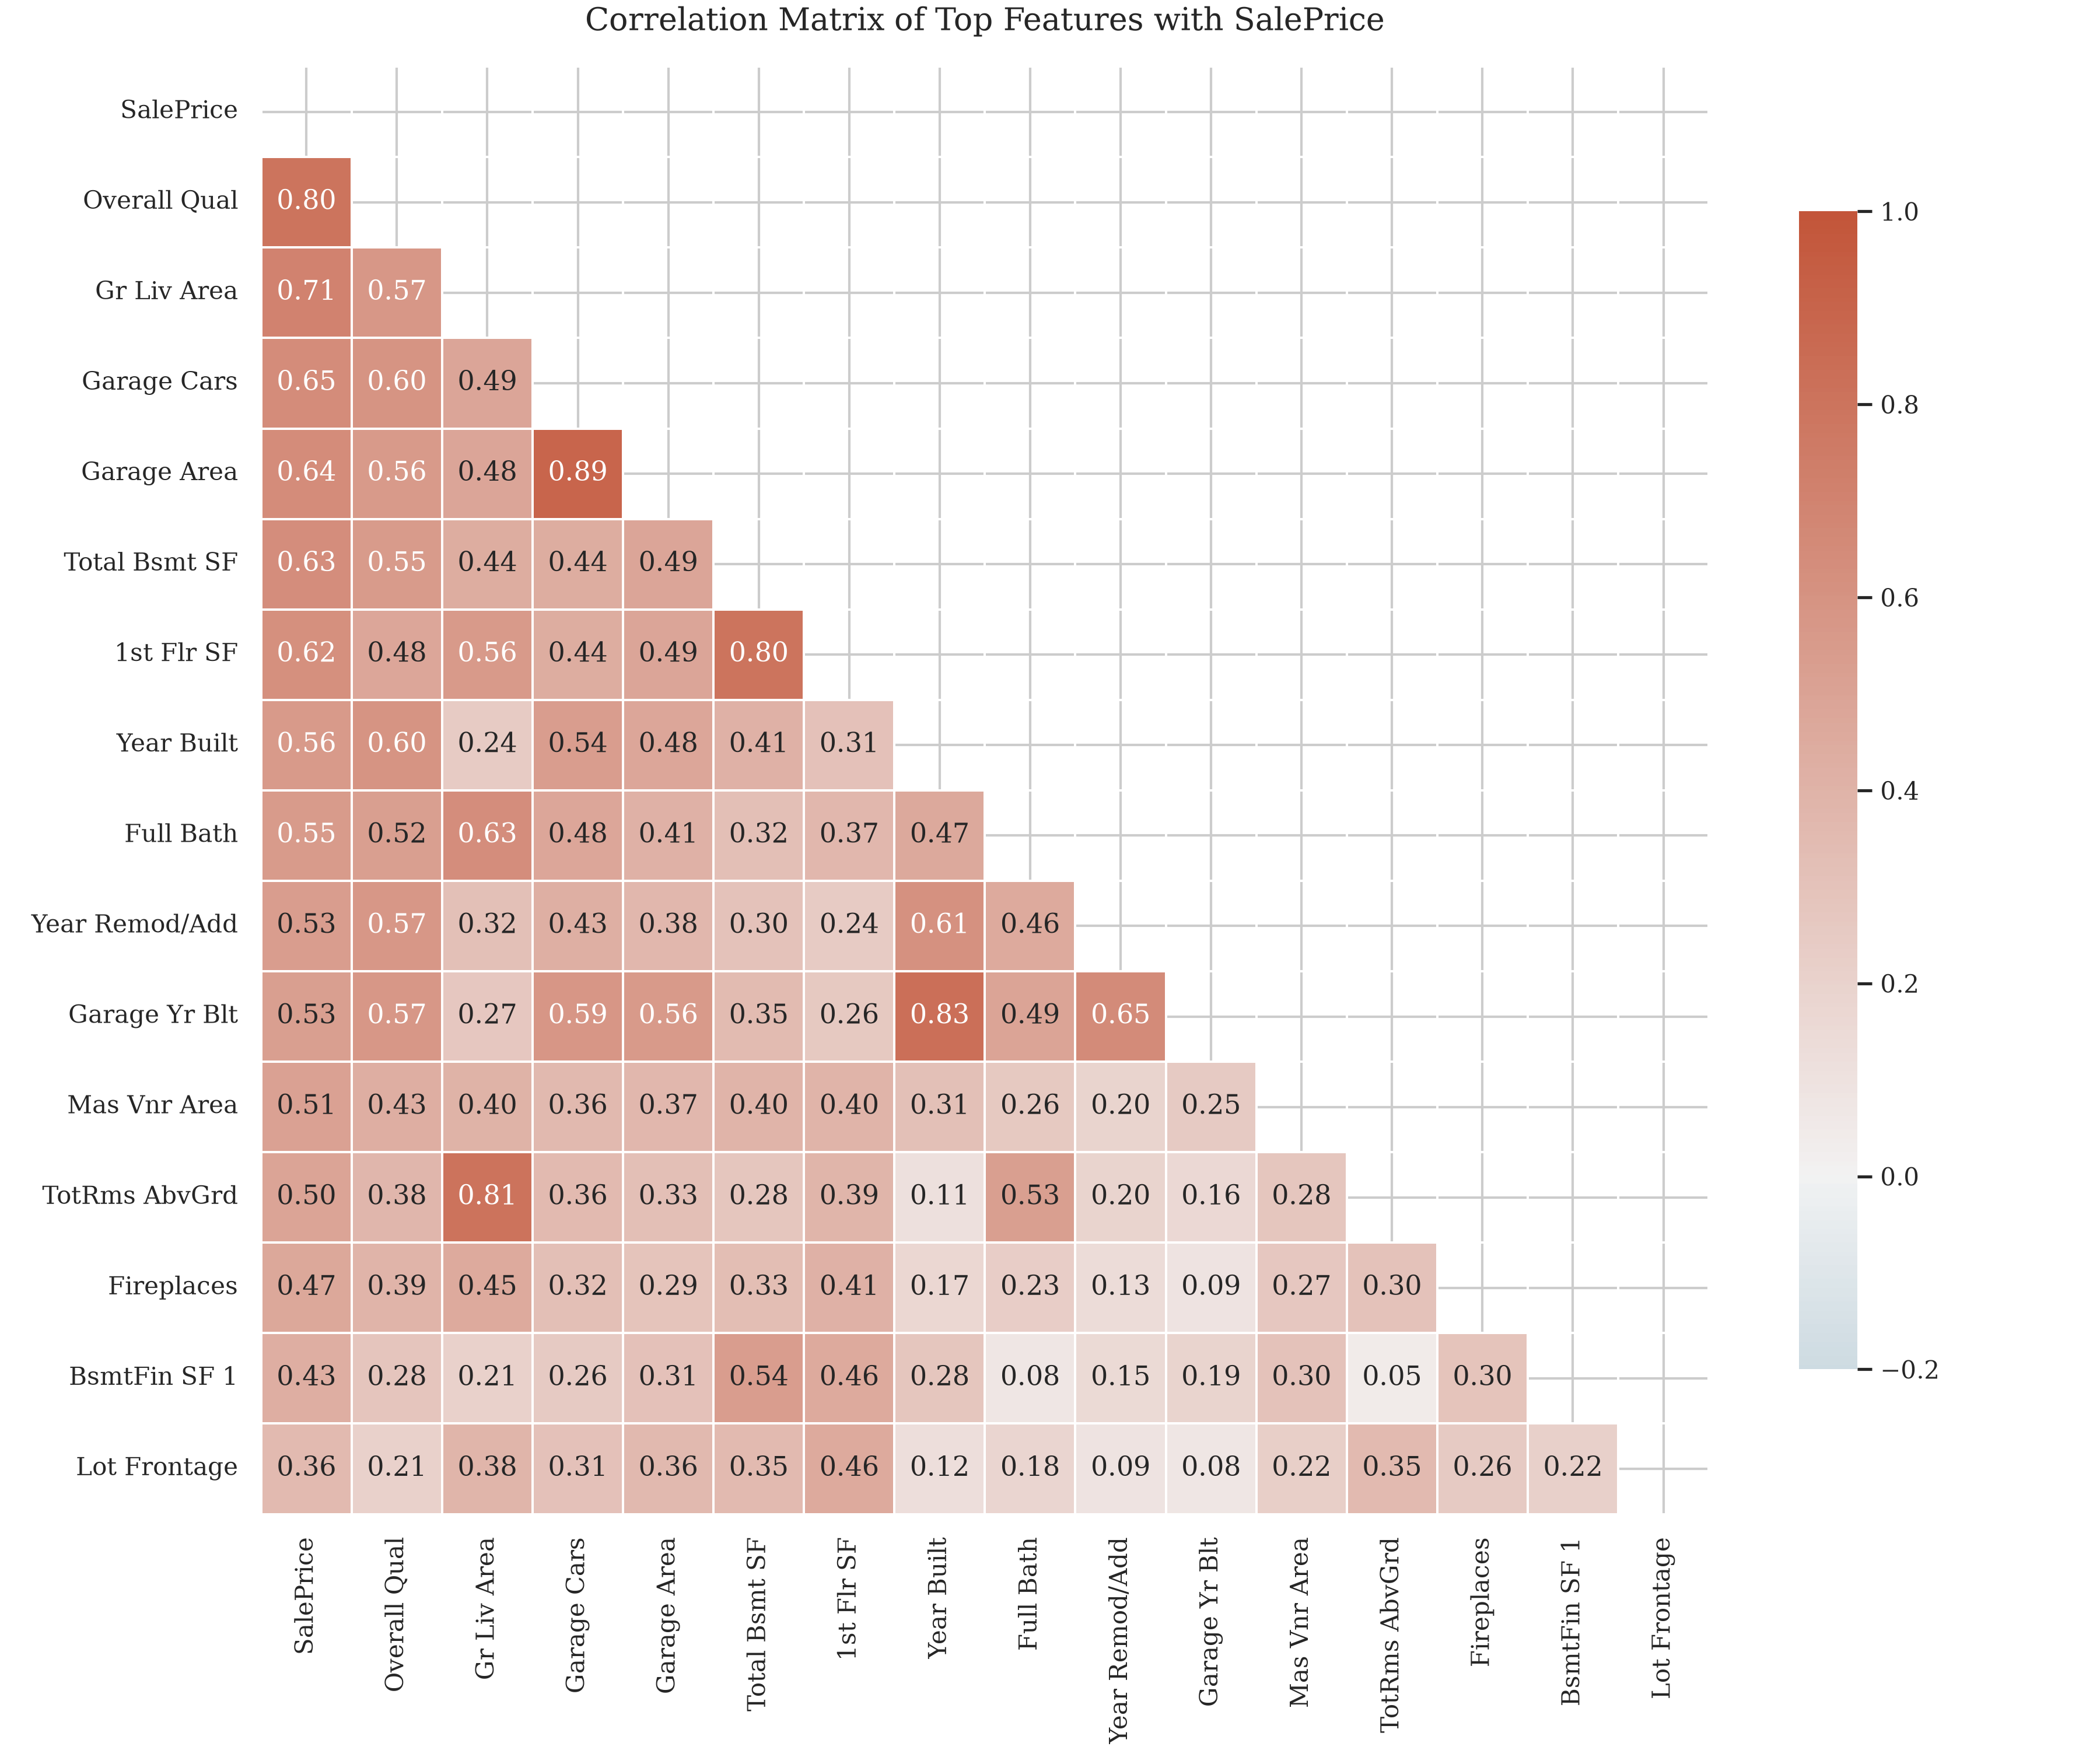
\includegraphics[width=0.78\textwidth]{../results/figures/correlation_heatmap.png}
\caption{Correlation matrix of top numerical predictors with \texttt{SalePrice}.}
\label{fig:correlation}
\end{figure}

Figure~\ref{fig:qual_and_neigh} shows the distribution of prices across categorical quality ratings (Overall Qual 1–10) and the median prices across Ames neighborhoods, highlighting spatial clustering where districts like Stone Brook (\texttt{StoneBr}) and Northridge Heights (\texttt{NridgHt}) trade at more than triple the median of Meadow Village (\texttt{MeadowV}).

\begin{figure}[H]
\centering
\begin{subfigure}[b]{0.48\textwidth}
    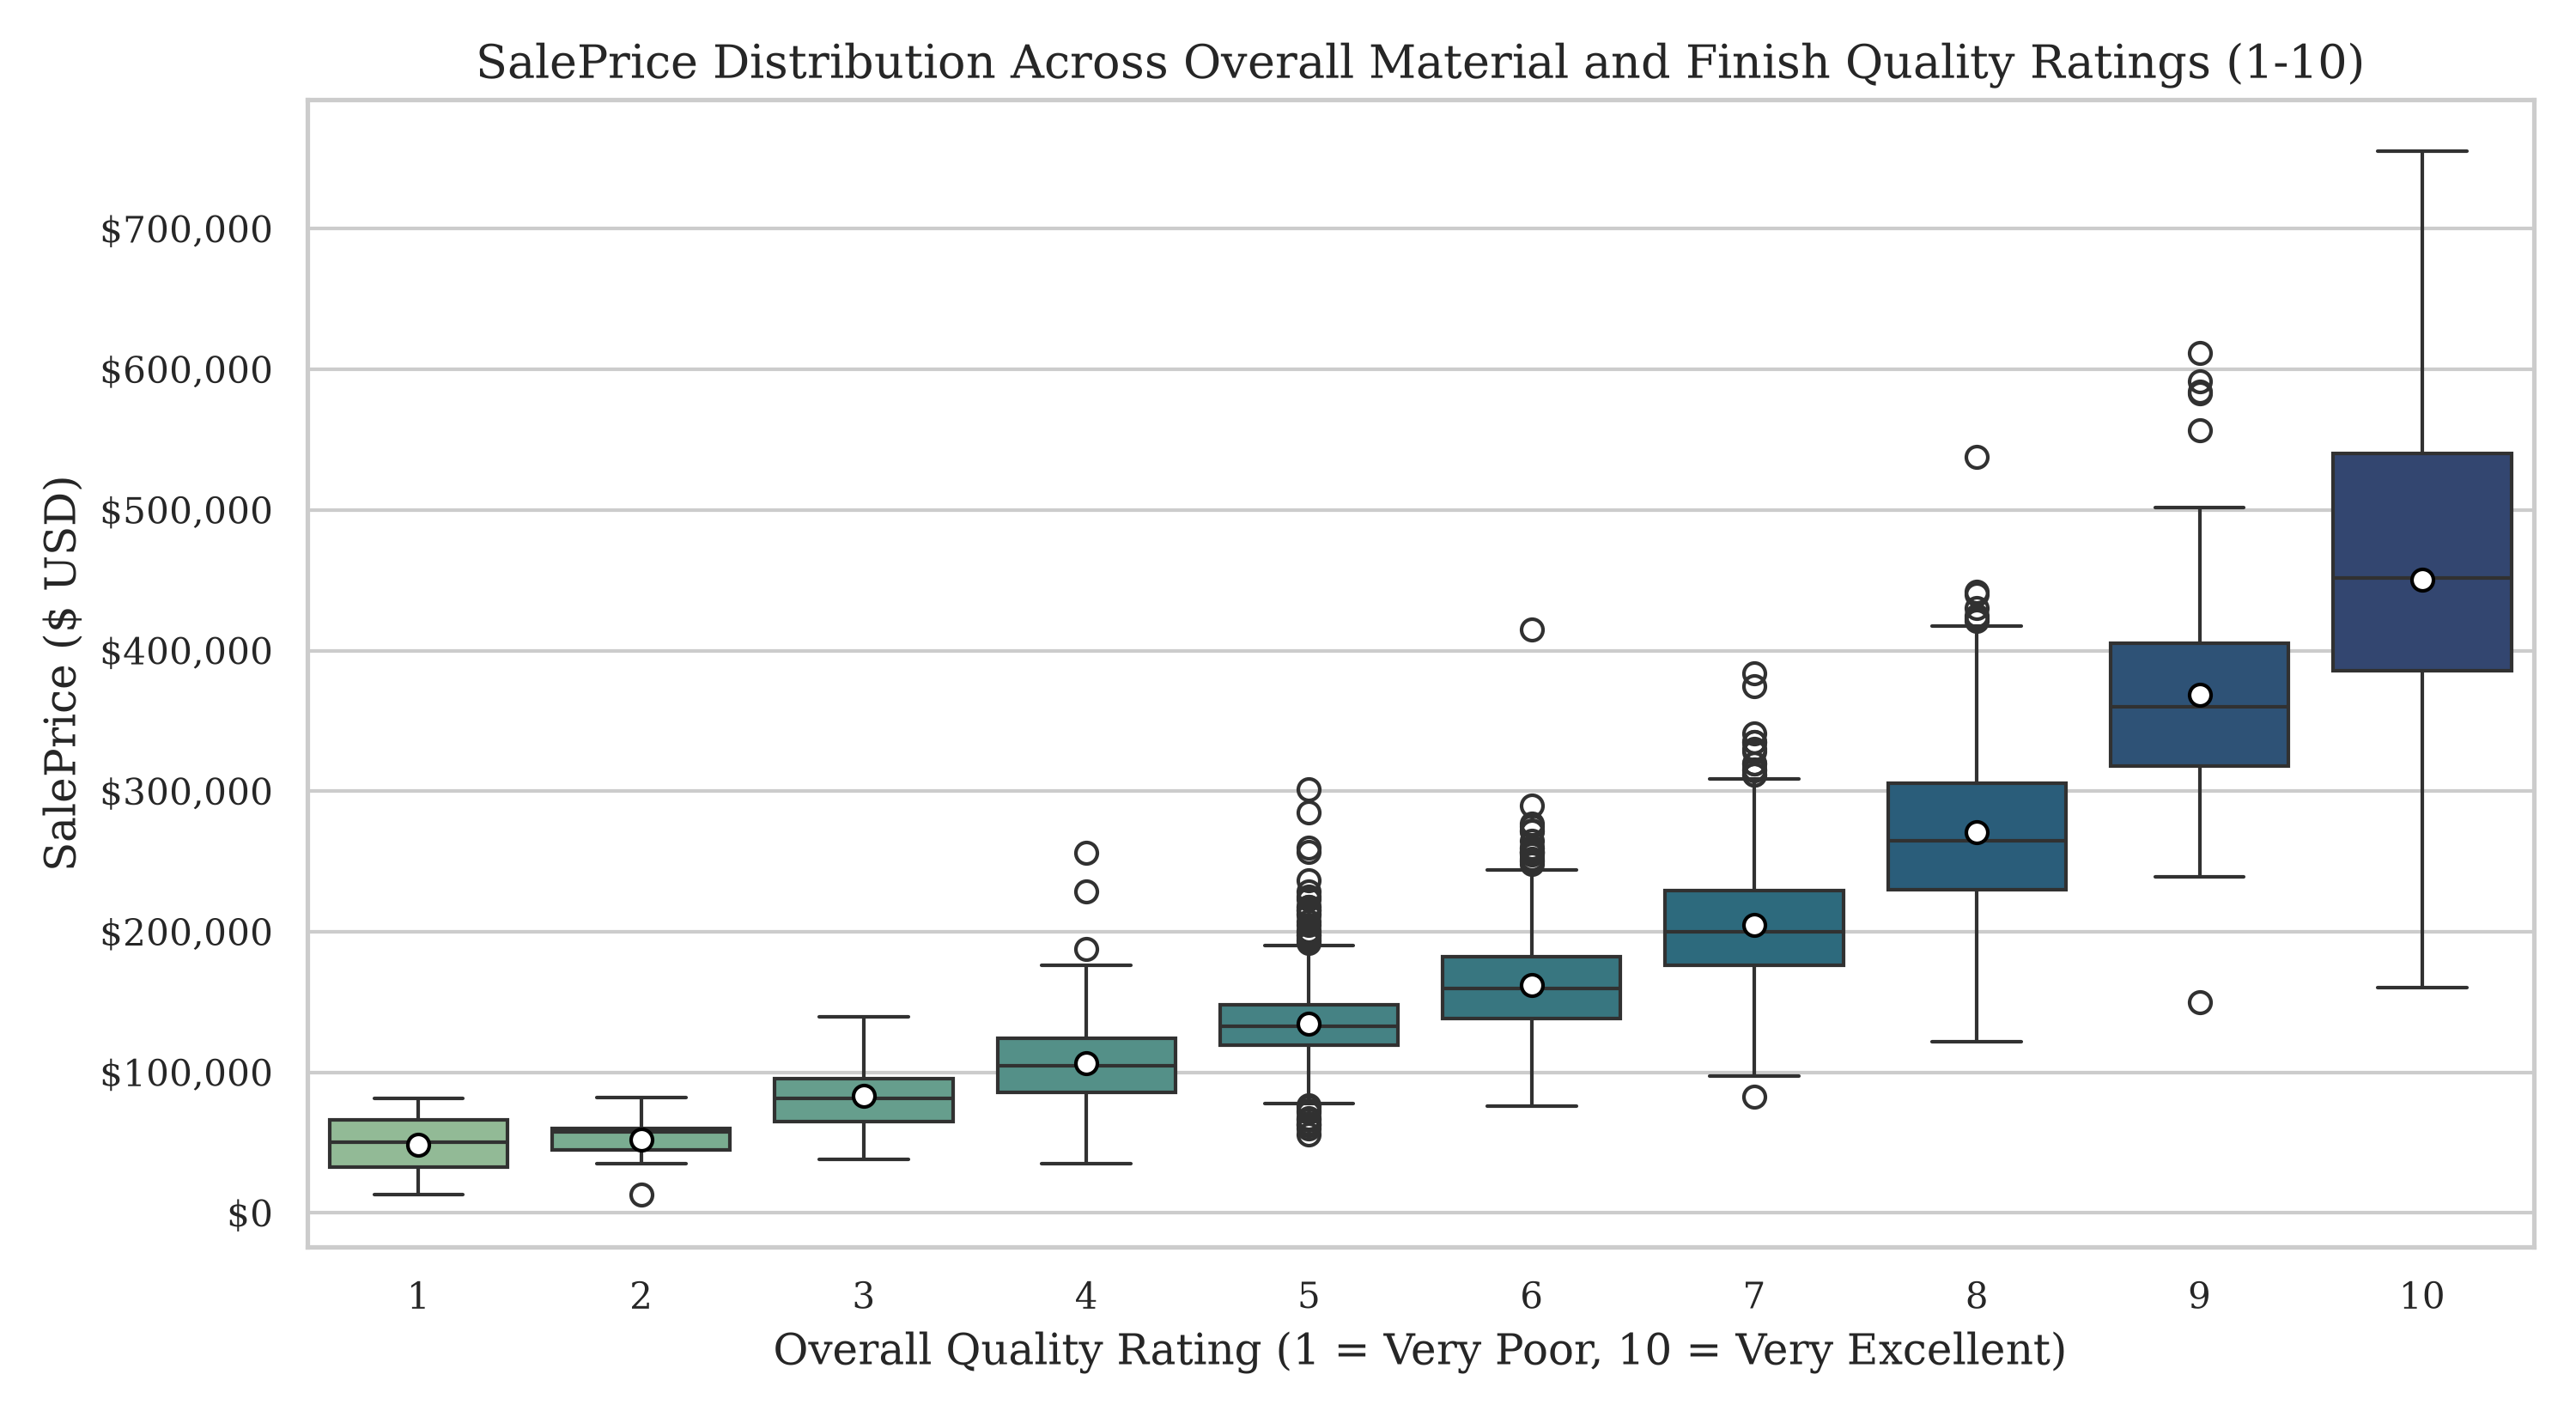
\includegraphics[width=\textwidth]{../results/figures/overall_qual_boxplot.png}
    \caption{Price distribution across Overall Quality (1–10).}
\end{subfigure}
\hfill
\begin{subfigure}[b]{0.48\textwidth}
    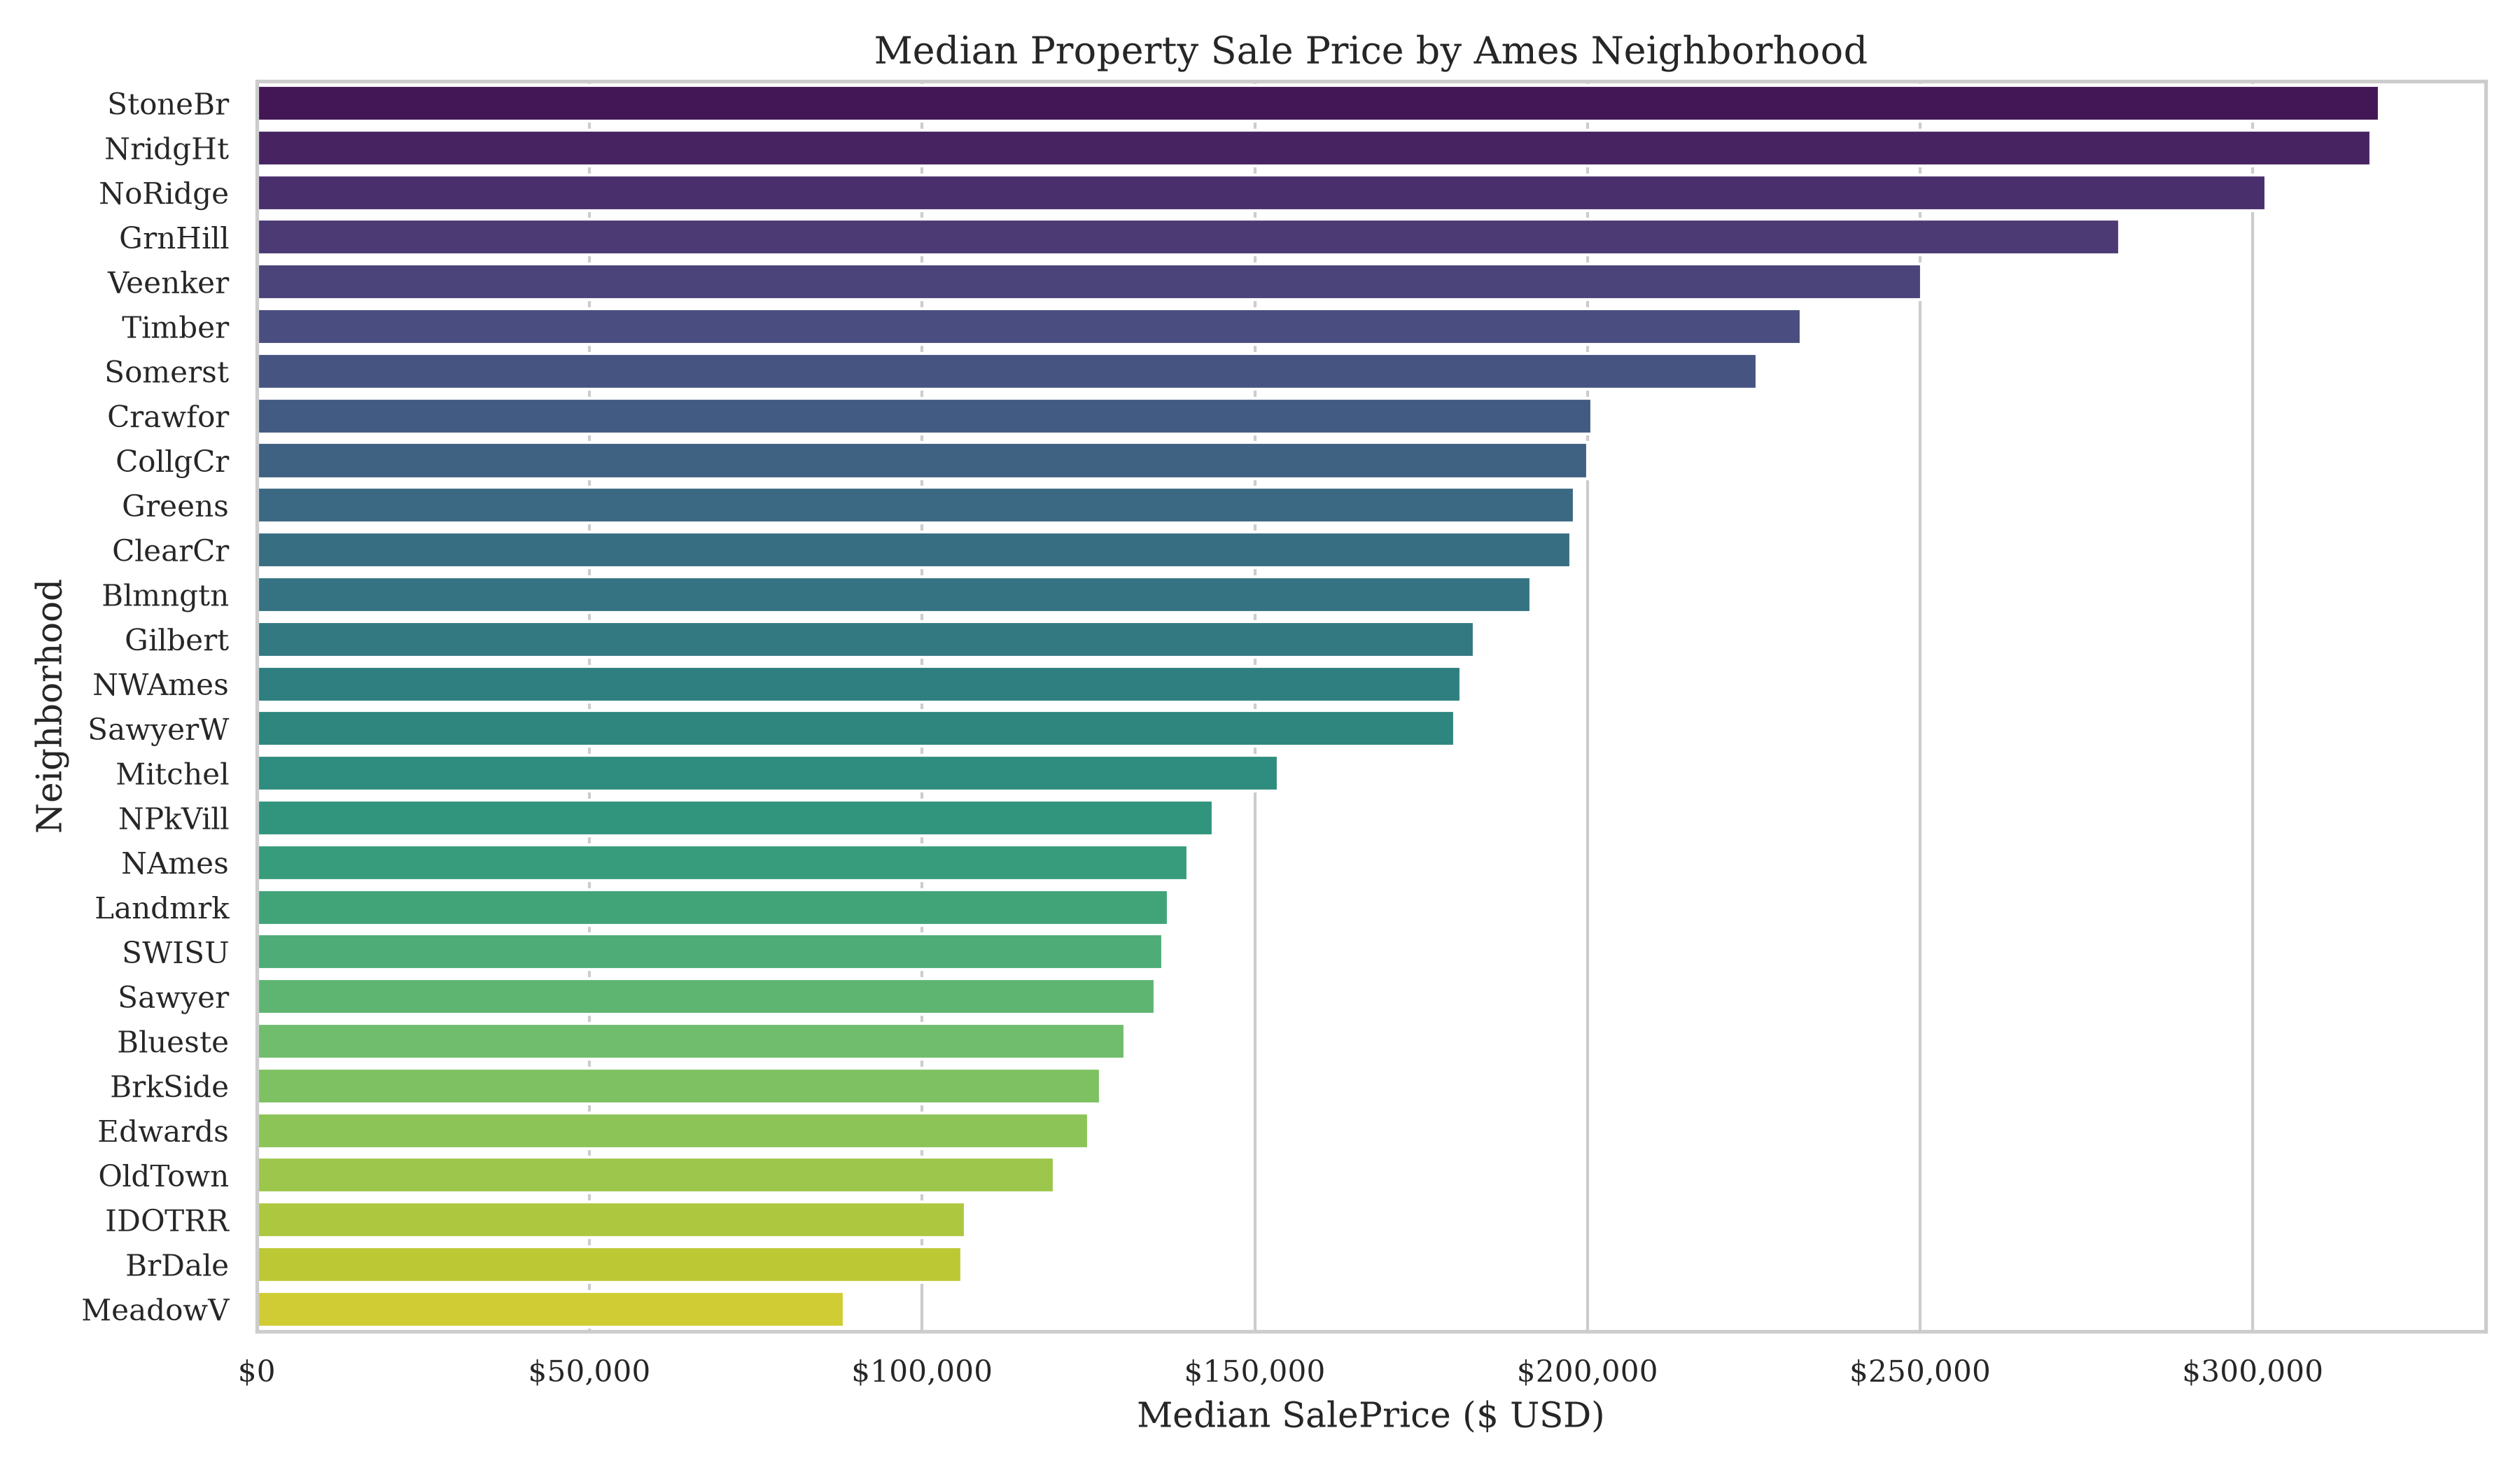
\includegraphics[width=\textwidth]{../results/figures/neighborhood_price.png}
    \caption{Median property price across Ames neighborhoods.}
\end{subfigure}
\caption{Valuation patterns across quality grades and spatial locations.}
\label{fig:qual_and_neigh}
\end{figure}

\section{Data Preprocessing Pipeline}
The preprocessing and feature engineering pipeline is implemented in \texttt{src/data\_loader.py} and \texttt{src/features.py}.

\subsection{Train/Validation/Test Partitioning Protocol}
To evaluate out-of-sample generalization without bias, we enforce a strict 70\% Train / 15\% Validation / 15\% Test partition using a fixed random seed (\texttt{random\_state=42}). The sample indices are saved to \texttt{data/splits.json}, ensuring exact reproducibility:
\begin{itemize}
    \item \textbf{Training Partition:} 2,050 samples (70.0\%)
    \item \textbf{Validation Partition:} 440 samples (15.0\%)
    \item \textbf{Testing Partition:} 440 samples (15.0\%)
\end{itemize}

\subsection{Domain Feature Engineering}
To provide baseline models with domain-relevant spatial representations, we engineered several composite features:
\begin{enumerate}
    \item \textbf{Total Usable Footprint (\texttt{TotalSF}):} $\text{TotalSF} = \text{Gr Liv Area} + \text{Total Bsmt SF}$. Combining above-ground and below-ground finished square footage yields a more comprehensive representation of living space ($r = 0.78$ with target).
    \item \textbf{Total Bathrooms (\texttt{TotalBath}):} $\text{TotalBath} = \text{FullBath} + 0.5 \times \text{HalfBath} + \text{BsmtFullBath} + 0.5 \times \text{BsmtHalfBath}$.
    \item \textbf{Property Age Metrics:} $\text{HouseAge} = \max(0, \text{Yr Sold} - \text{Year Built})$ and $\text{RemodAge} = \max(0, \text{Yr Sold} - \text{Year Remod/Add})$. An indicator $\text{IsRemodeled} = \mathbb{I}(\text{Year Remod/Add} \neq \text{Year Built})$ tracks structural modernization.
    \item \textbf{Total Outdoor Decking (\texttt{TotalPorchSF}):} Sum of Wood Deck, Open Porch, Enclosed Porch, 3-Season Porch, and Screen Porch.
    \item \textbf{Amenity Presence Indicators:} Binary flags $\text{HasPool}$, $\text{HasGarage}$, $\text{HasFireplace}$, and $\text{HasBsmt}$.
    \item \textbf{Quality Interaction:} $\text{OverallScore} = \text{Overall Qual} \times \text{Overall Cond}$.
\end{enumerate}

\subsection{Categorical Encoding and Feature Scaling}
\begin{itemize}
    \item \textbf{Ordinal Encoding:} Features with ordered assessments (\texttt{Exter Qual}, \texttt{Bsmt Qual}, \texttt{Kitchen Qual}, \texttt{Fireplace Qu}, \texttt{Heating QC}, \texttt{Garage Qual}, \texttt{Pool QC}) are mapped monotonically: $\text{Ex} \to 5$, $\text{Gd} \to 4$, $\text{TA} \to 3$, $\text{Fa} \to 2$, $\text{Po} \to 1$, $\text{None} \to 0$.
    \item \textbf{Nominal One-Hot Encoding:} Categorical features without natural ordering (\texttt{Neighborhood}, \texttt{Bldg Type}, \texttt{MS Zoning}, \texttt{Foundation}, etc.) are encoded using Scikit-Learn's \texttt{OneHotEncoder} configured with \texttt{handle\_unknown='ignore'}.
    \item \textbf{Robust Scaling:} Continuous features are normalized with \texttt{RobustScaler()}, which centers each attribute at the training median and scales by the interquartile range ($IQR$), providing resistance to skewed features.
\end{itemize}
The final representation comprises \textbf{260 encoded features}.

\subsection{Data Leakage Prevention}
Data leakage is rigorously prevented through the following controls:
\begin{enumerate}
    \item The preprocessor computes neighborhood medians, categorical modes, and scaling quantiles \textbf{exclusively on the training partition}.
    \item Outlier removal ($>4,000$ sq ft) is executed \textbf{only on the training split} during fitting. The validation and test sets remain unpruned to preserve real-world evaluation integrity.
    \item During inference, unknown categorical levels encountered in test data are mapped to all-zero dummy vectors via \texttt{handle\_unknown='ignore'}.
\end{enumerate}

\section{Supervised Baseline Models and Evaluation}
We implemented, trained, and validated three distinct baseline models in \texttt{src/baselines.py}:
\begin{enumerate}
    \item \textbf{Baseline 1 — Regularized Linear Regression (Ridge):} Applies an $L_2$ penalty to control multicollinearity across the 260 engineered features. Hyperparameter optimization via 5-fold cross-validation on the training set identified $\alpha^* = 29.47$.
    \item \textbf{Baseline 2 — Random Forest Regressor:} An ensemble of 250 randomized decision trees (\texttt{max\_depth=22}, \texttt{min\_samples\_split=4}, \texttt{min\_samples\_leaf=2}, \texttt{random\_state=42}).
    \item \textbf{Baseline 3 — Gradient Boosting Regressor (GBR):} An ensemble of 250 sequentially boosted decision stumps (\texttt{learning\_rate=0.05}, \texttt{max\_depth=4}, \texttt{subsample=0.85}, \texttt{random\_state=42}) trained to minimize mean squared error in log-space.
\end{enumerate}

\subsection{Empirical Benchmark Results}
Table~\ref{tab:model_comparison} summarizes model performance across the Train, Validation, and Test partitions. Metrics are reported in both real currency (MAE and RMSE in USD) and log-scale (RMSLE).

\begin{table}[H]
\centering
\small
\caption{Comprehensive Performance Benchmark of Supervised Baseline Models}
\label{tab:model_comparison}
\begin{tabular}{llrrrr}
\toprule
\textbf{Model} & \textbf{Split} & \textbf{MAE (\$ USD)} & \textbf{RMSE (\$ USD)} & \textbf{$R^2$ Score} & \textbf{RMSLE (log)} \\
\midrule
\textbf{Ridge Regression}   & Train      & \$12,508.91 & \$18,368.79 & 0.9417 & 0.1094 \\
($\alpha = 29.47$)          & Validation & \$14,101.86 & \$20,057.30 & 0.9481 & 0.1156 \\
                            & \textbf{Test} & \textbf{\$15,031.51} & \textbf{\$44,511.47} & \textbf{0.7421} & \textbf{0.1254} \\
\midrule
\textbf{Random Forest}      & Train      & \$6,279.71  & \$10,485.18 & 0.9810 & 0.0604 \\
(250 Trees, max depth 22)   & Validation & \$17,779.07 & \$28,992.06 & 0.8916 & 0.1384 \\
                            & \textbf{Test} & \textbf{\$16,700.76} & \textbf{\$31,325.66} & \textbf{0.8723} & \textbf{0.1325} \\
\midrule
\textbf{Gradient Boosting}  & Train      & \$7,878.73  & \$10,739.24 & 0.9801 & 0.0591 \\
(250 Trees, lr = 0.05)      & Validation & \$14,963.25 & \$22,986.39 & 0.9319 & 0.1199 \\
                            & \textbf{Test} & \textbf{\$14,876.80} & \textbf{\$31,939.29} & \textbf{0.8672} & \textbf{0.1208} \\
\bottomrule
\end{tabular}
\end{table}

\subsection{Diagnostic Residual and Fit Analysis}
Figure~\ref{fig:actual_vs_pred} illustrates the Actual vs. Predicted \texttt{SalePrice} on the unseen Test set ($N = 440$). All three baselines track the ideal $y = x$ trajectory across typical home prices (\$100,000–\$350,000). Ridge Regression experiences higher variance on extreme luxury homes, which inflates its raw-dollar RMSE to \$44,511.47, despite maintaining a competitive MAE of \$15,031.51 and an RMSLE of 0.1254.

\begin{figure}[H]
\centering
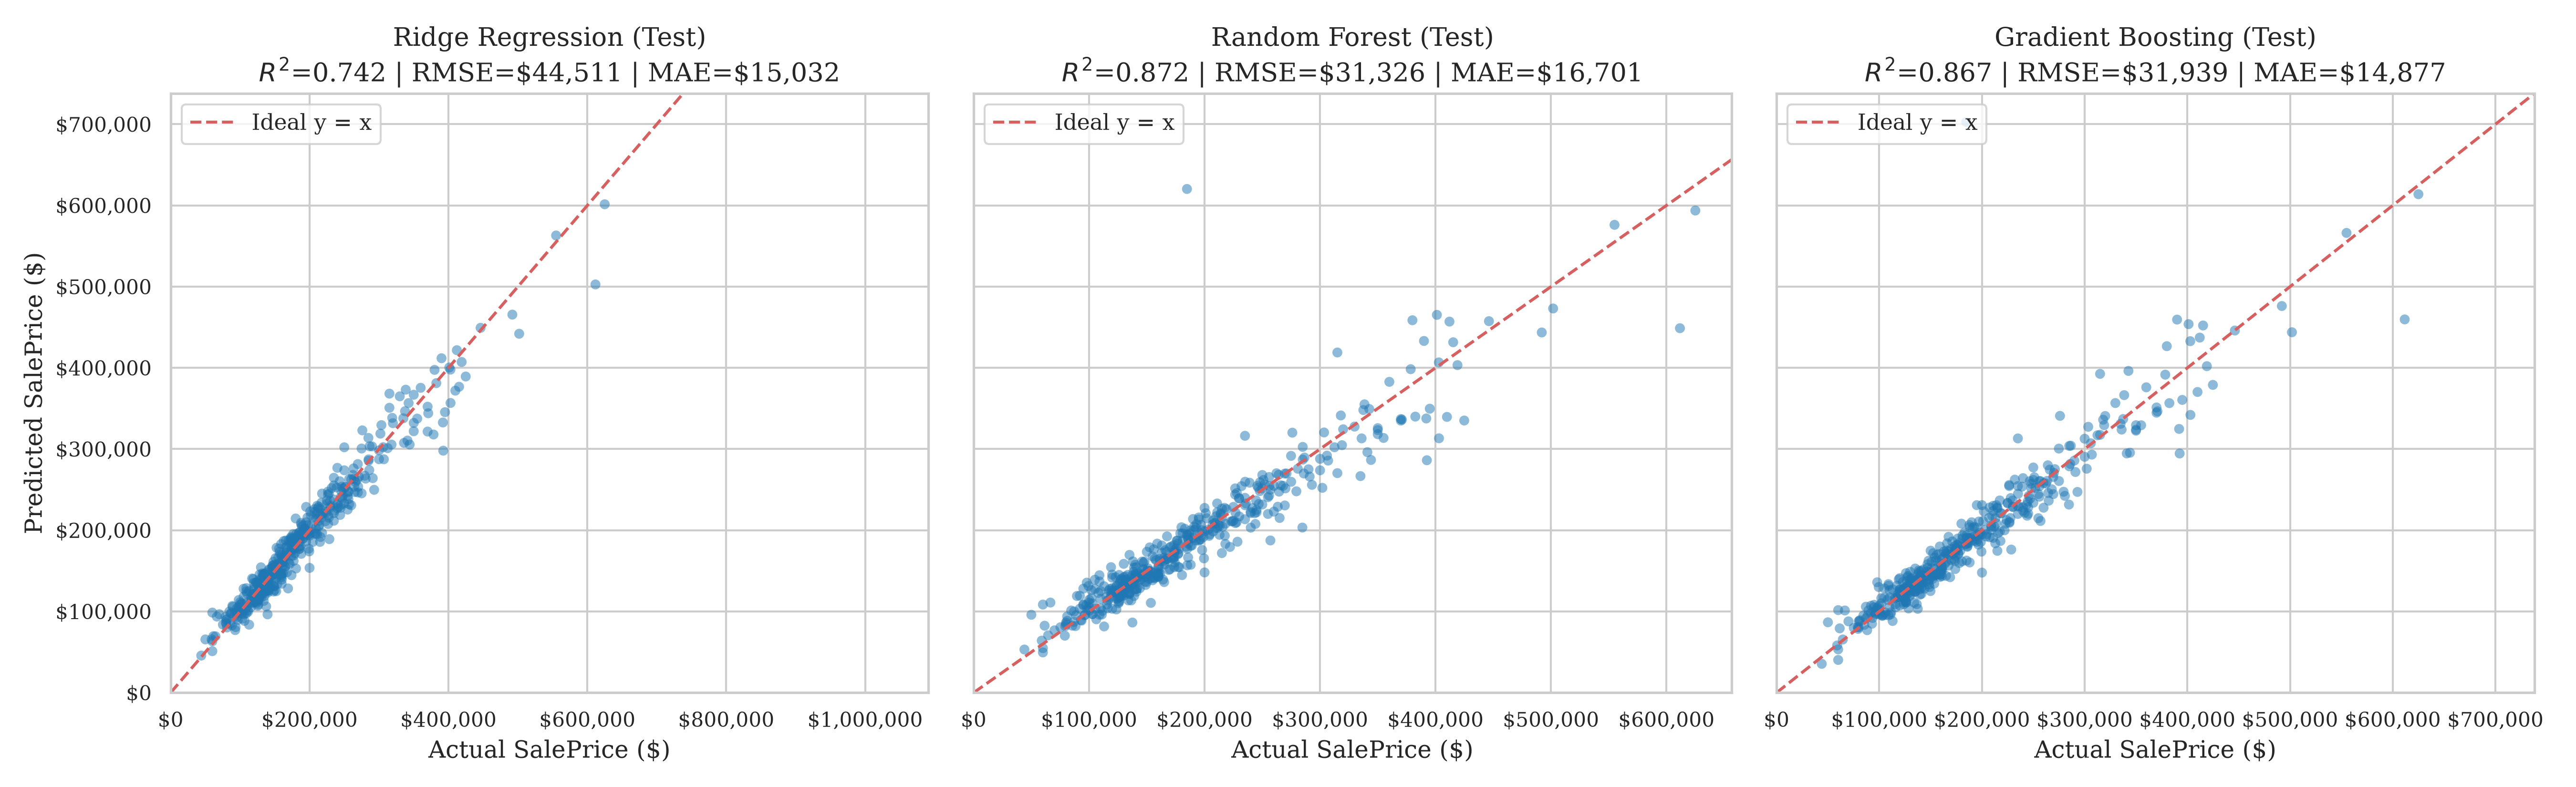
\includegraphics[width=\textwidth]{../results/figures/actual_vs_predicted.png}
\caption{Actual vs. Predicted \texttt{SalePrice} on the held-out Test set ($N = 440$) for Ridge, Random Forest, and Gradient Boosting.}
\label{fig:actual_vs_pred}
\end{figure}

Figure~\ref{fig:residuals_and_dist} displays the residual scatter plots and error distributions. The residuals are centered near zero ($\mu \approx \$0$) with approximate normality, confirming the variance stabilization achieved by modeling in $\log(1 + y)$ space.

\begin{figure}[H]
\centering
\begin{subfigure}[b]{0.95\textwidth}
    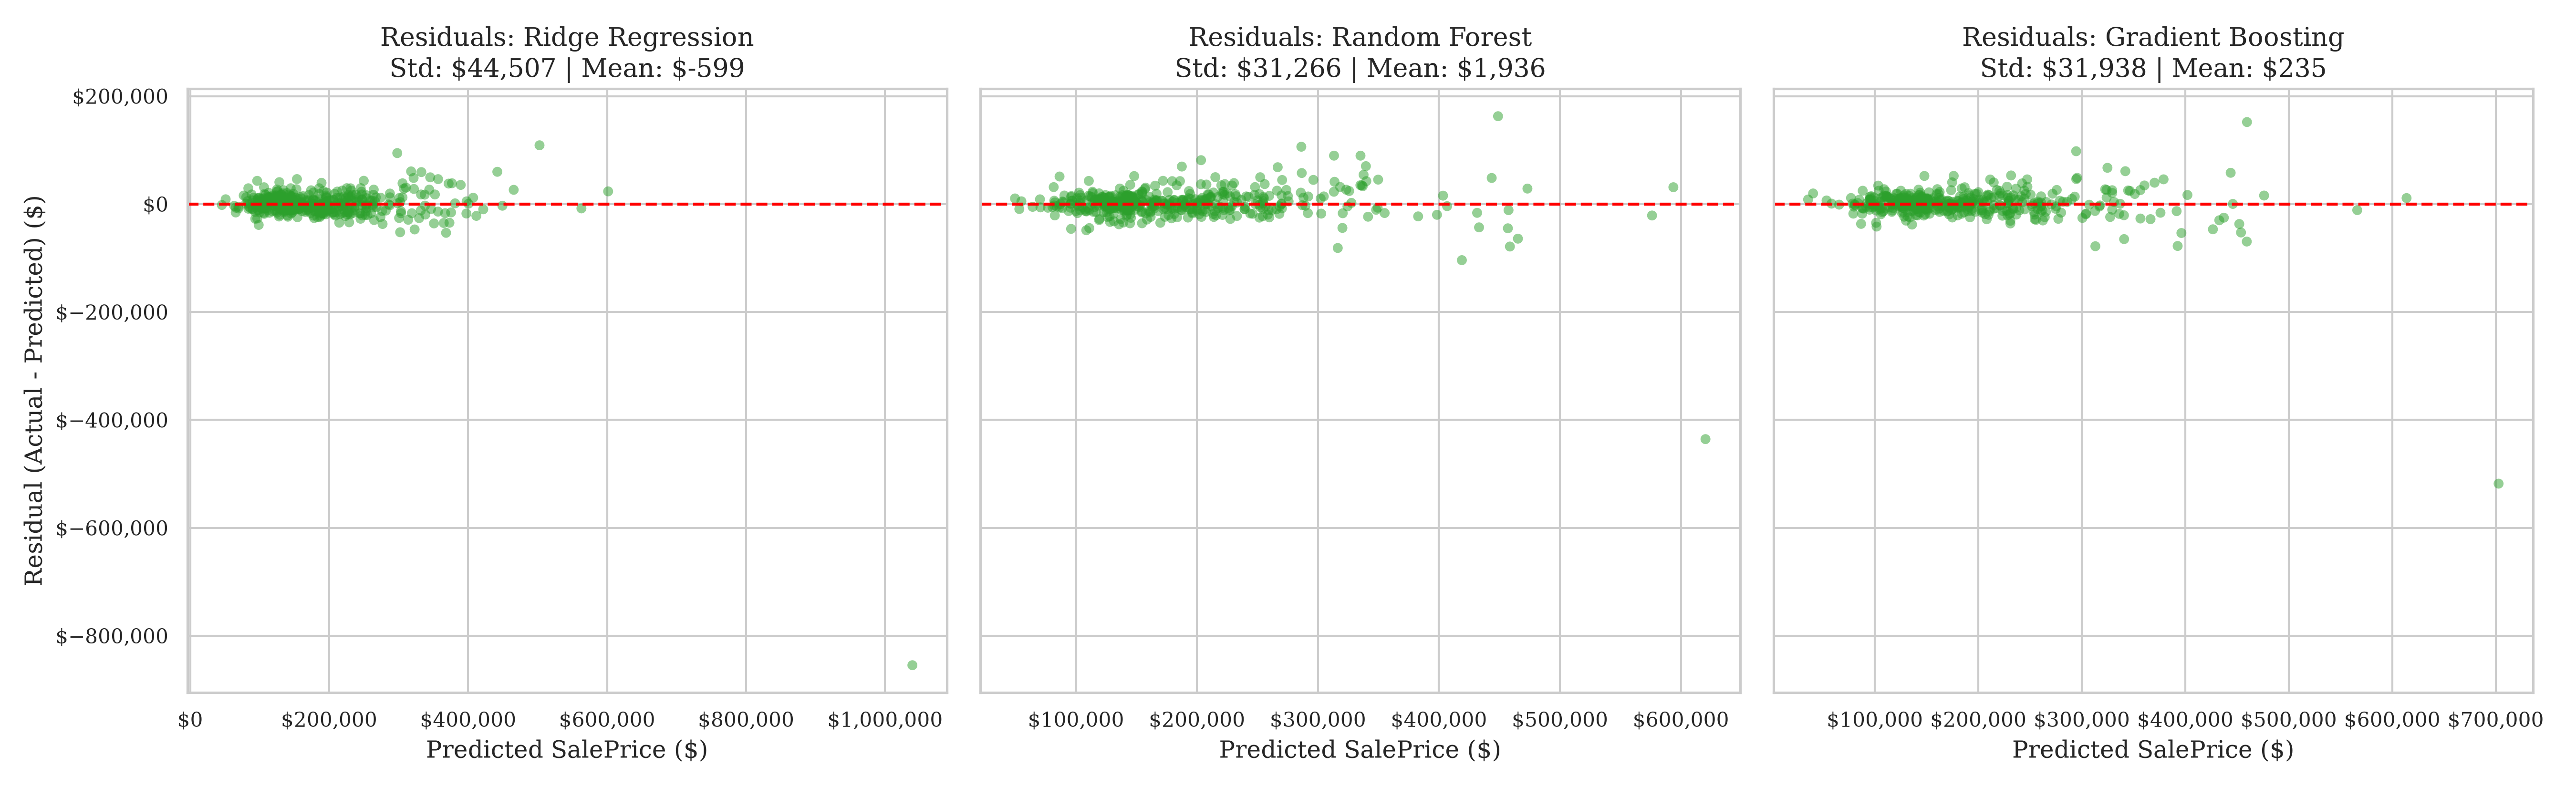
\includegraphics[width=\textwidth]{../results/figures/residuals_plot.png}
    \caption{Residuals vs. Predicted Values on the held-out Test set.}
\end{subfigure}
\vspace{0.3cm}
\begin{subfigure}[b]{0.95\textwidth}
    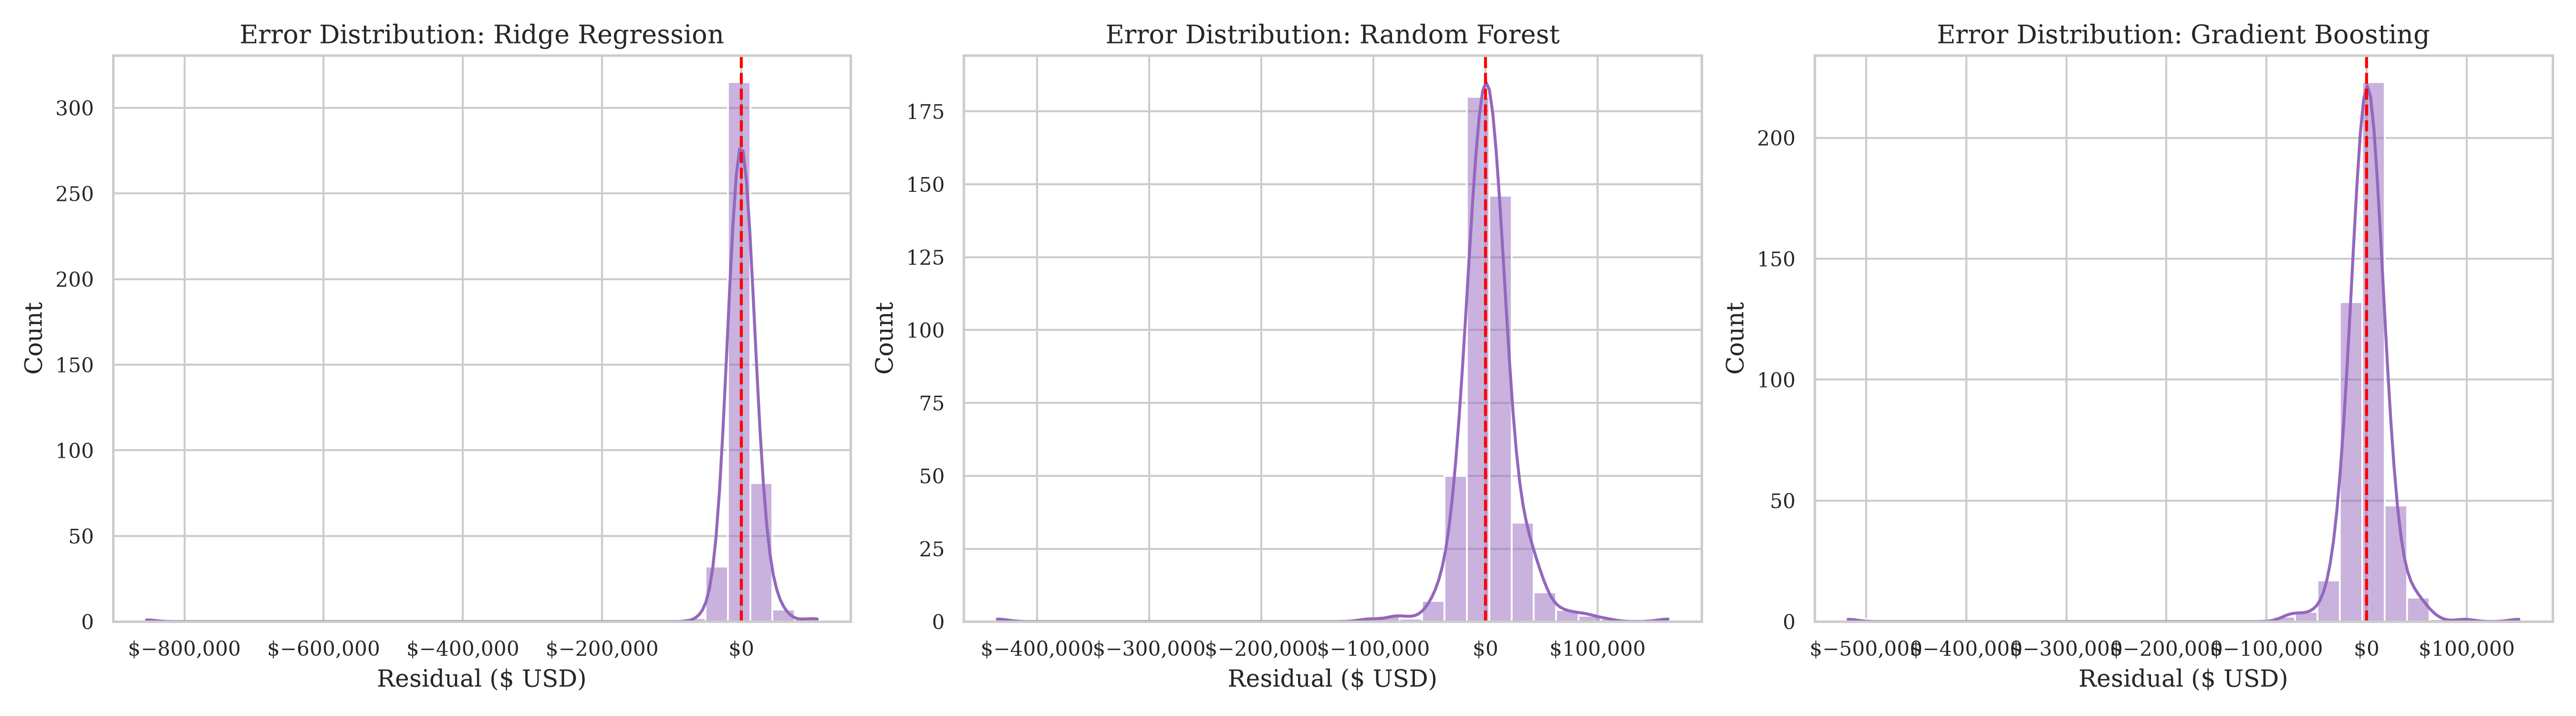
\includegraphics[width=\textwidth]{../results/figures/residuals_distribution.png}
    \caption{Error distributions (Residuals in USD) across all three baseline models.}
\end{subfigure}
\caption{Residual diagnostic plots assessing homoscedasticity and normality on the Test set.}
\label{fig:residuals_and_dist}
\end{figure}

\subsection{Feature Importance Analysis}
Figure~\ref{fig:feat_importance} visualizes the top 15 predictors identified by Random Forest and Gradient Boosting. Both models identify \texttt{Overall Qual}, total usable footprint (\texttt{TotalSF}), above-ground living area (\texttt{Gr Liv Area}), and basement finished space (\texttt{BsmtFin SF 1}) as the most informative predictors, confirming the value of the engineered composite features.

\begin{figure}[H]
\centering
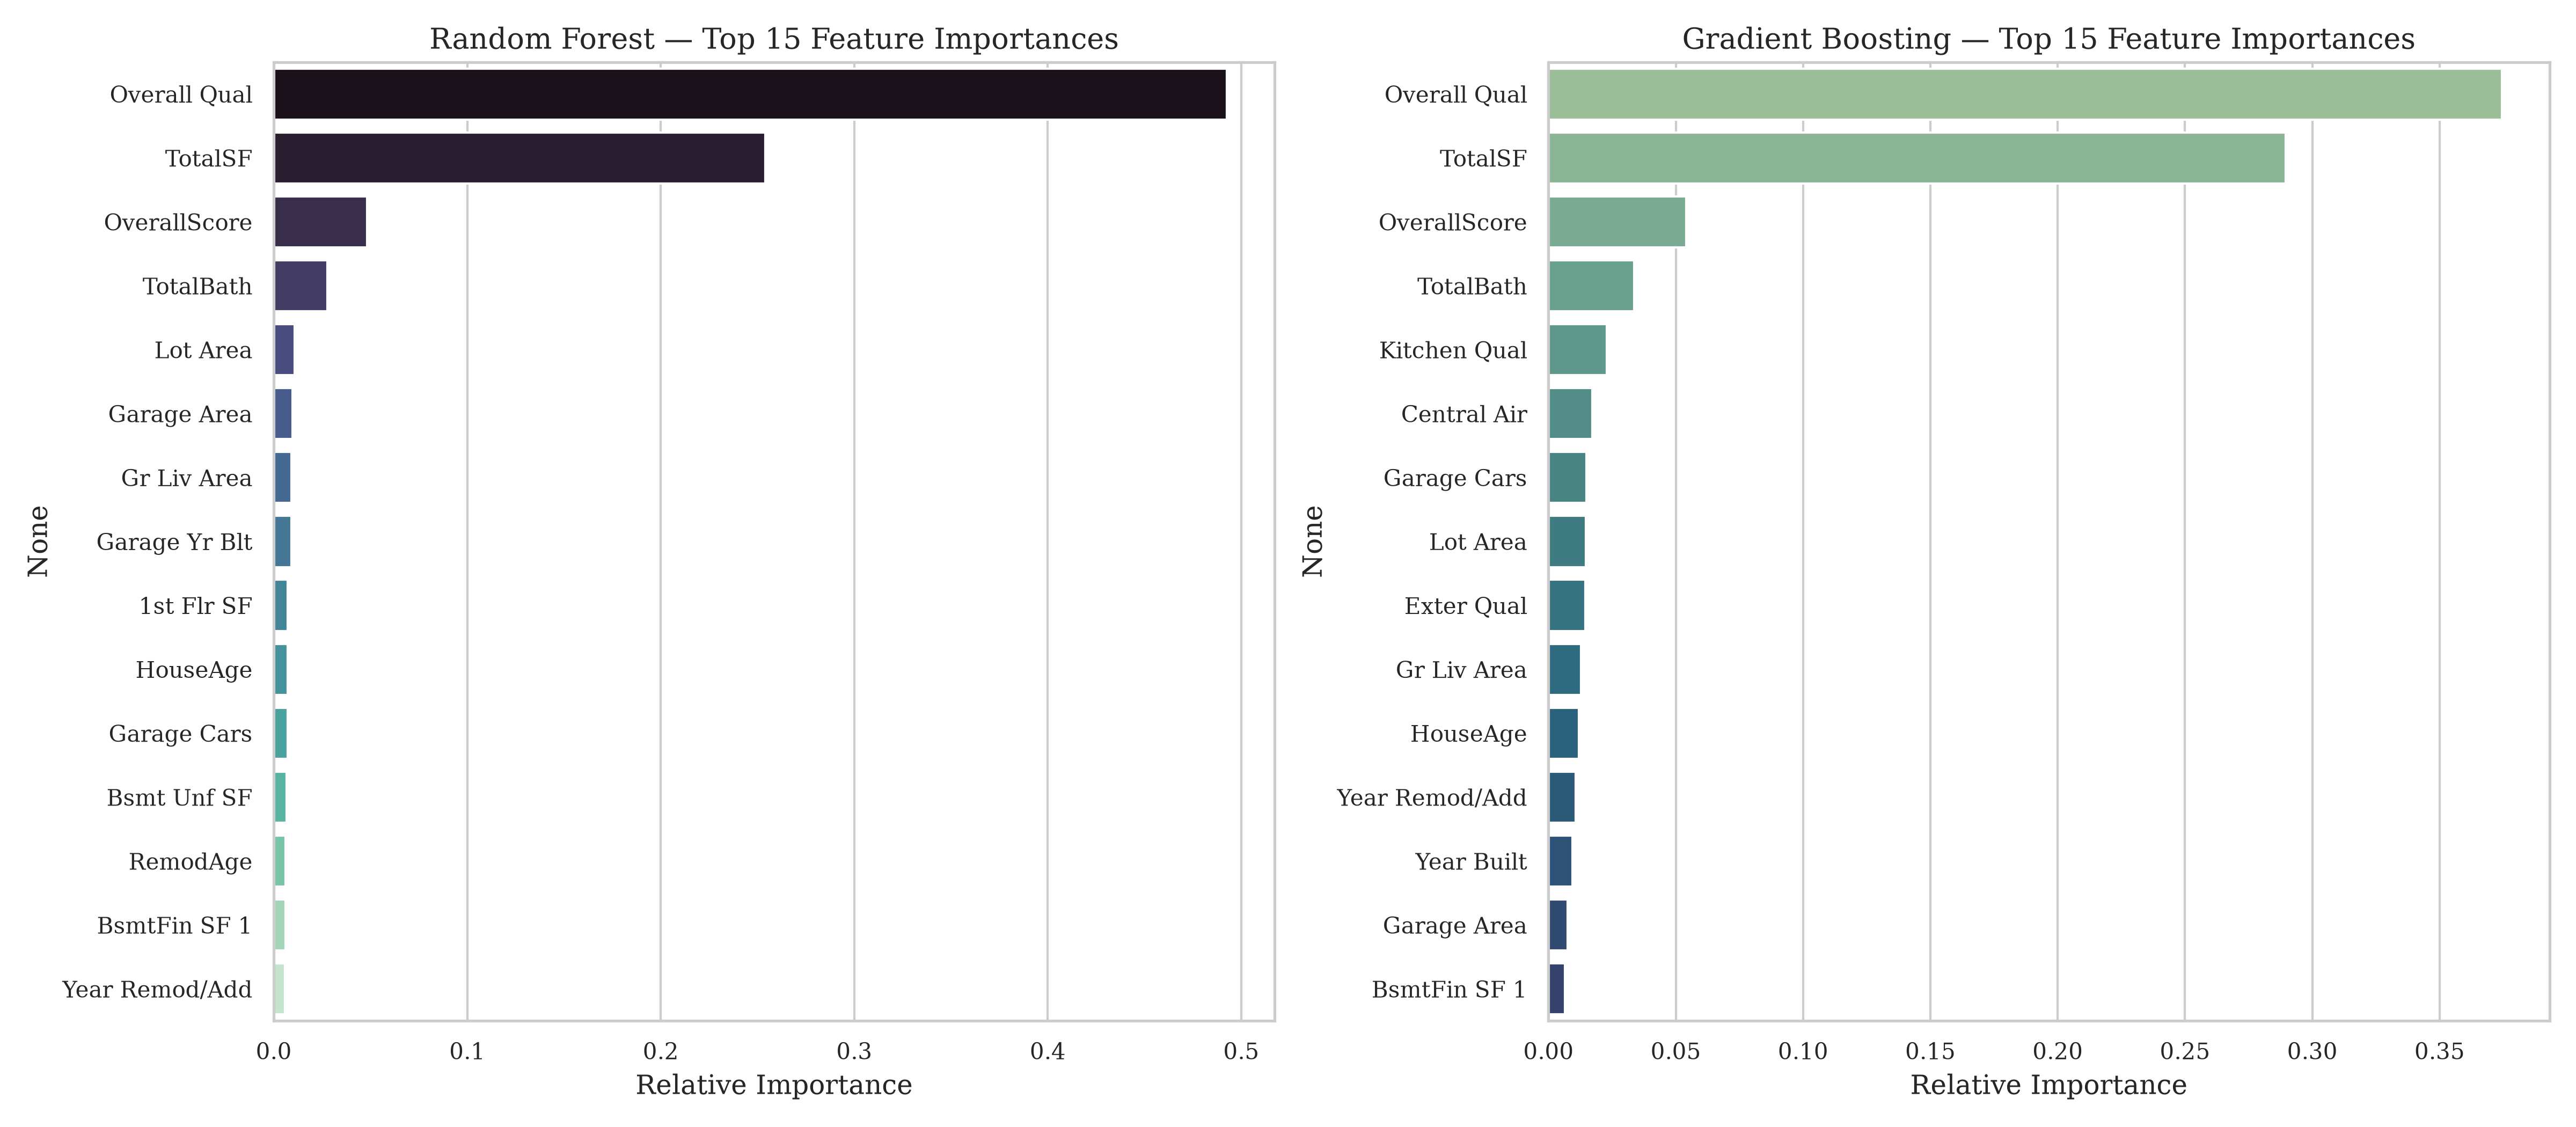
\includegraphics[width=0.92\textwidth]{../results/figures/feature_importance.png}
\caption{Top 15 feature importances extracted from Random Forest and Gradient Boosting Regressors.}
\label{fig:feat_importance}
\end{figure}

\section{Discussion and Critical Insights}

\subsection{Problem Difficulty and Evaluation Metric Selection}
Real estate pricing is characterized by high variance: two homes with identical square footage and room counts may trade at substantially different valuations due to micro-locational differences (cul-de-sac vs. arterial road) and unobserved subjective aesthetics. 

Our benchmark results highlight important nuances in metric selection:
\begin{itemize}
    \item \textbf{RMSE Sensitivity:} In raw dollar space, RMSE heavily penalizes large errors on luxury estates ($>\$500,000$). For example, a 10\% prediction error on a \$600,000 property contributes \$3.6 billion to squared error, whereas the same 10\% error on a \$120,000 starter home contributes only \$144 million. This disparity explains why Ridge Regression exhibits an elevated Test RMSE (\$44,511.47) despite achieving an MAE (\$15,031.51) and RMSLE (0.1254) comparable to Gradient Boosting.
    \item \textbf{MAE and RMSLE Suitability:} For real estate valuation, MAE and RMSLE provide more reliable and interpretable measures of expected error across property tiers. Gradient Boosting's test RMSLE of \textbf{0.1208} indicates that on average, baseline predictions fall within approximately $12\%$ of actual property sale value.
\end{itemize}

\subsection{Comparison of Model Paradigms}
\begin{itemize}
    \item \textbf{Ridge Regression:} Demonstrates strong computational efficiency and benefits from regularized shrinkage across the 260 features. However, its linear functional form cannot directly capture complex non-linear land-to-building interactions without extensive manual polynomial expansions.
    \item \textbf{Random Forest:} Reduces variance through bagging, delivering steady predictions across the median price range. However, decision tree averaging tends to underpredict top-tier luxury valuations due to bounded leaf predictions.
    \item \textbf{Gradient Boosting:} Achieves the strongest overall performance ($\text{Test MAE} = \$14,876.80$, $\text{RMSLE} = 0.1208$). By optimizing pseudo-residuals sequentially with shrinkage ($\eta = 0.05$) and stochastic row sampling ($0.85$), it captures subtle feature interactions while avoiding over-reliance on individual high-leverage samples.
\end{itemize}

\subsection{Key Implications for Workshop 2 (Deep Learning)}
These classical machine learning baselines establish several key foundations for future workshops:
\begin{enumerate}
    \item \textbf{Target Transformation:} Logarithmic target modeling is essential to stabilize gradient backpropagation and prevent exploding loss values from high-end properties.
    \item \textbf{Entity Embeddings for High-Cardinality Categoricals:} Deep architectures (e.g., Multilayer Perceptrons and TabNet) will benefit from dense entity embeddings for features like \texttt{Neighborhood} and \texttt{MSSubClass}, replacing sparse one-hot representations.
    \item \textbf{Performance Reference Anchor:} Gradient Boosting's Test $\text{MAE} = \$14,876.80$ and $\text{RMSLE} = 0.1208$ serve as the formal reference benchmarks that deep learning models must aim to surpass.
\end{enumerate}

\section*{Repository and Reproducibility Notice}
All artifacts, source modules, and data splits are committed to the course repository:
\begin{itemize}
    \item \textbf{Data Loader and Splitting:} \texttt{workshop1\_supervised/src/data\_loader.py}
    \item \textbf{Feature Pipeline:} \texttt{workshop1\_supervised/src/features.py}
    \item \textbf{Supervised Baselines:} \texttt{workshop1\_supervised/src/baselines.py}
    \item \textbf{Integrity Scanner:} \texttt{workshop1\_supervised/src/dataset\_info.py}
    \item \textbf{Exploratory Analysis:} \texttt{workshop1\_supervised/notebooks/eda.ipynb}
    \item \textbf{Deterministic Splits:} \texttt{data/splits.json}
\end{itemize}

To reproduce all results from scratch:
\begin{verbatim}
# 1. Activate environment
venv\Scripts\activate

# 2. Verify dataset integrity
python workshop1_supervised/src/dataset_info.py

# 3. Train all baselines and generate figures
python workshop1_supervised/src/baselines.py
\end{verbatim}

\begin{thebibliography}{9}
\bibitem{decock2011}
De Cock, D. (2011). 
\textit{Ames, Iowa: Alternative to the Boston Housing Data as an End of Semester Regression Project}. 
Journal of Statistics Education, 19(3). \url{https://doi.org/10.1080/10691898.2011.11889627}.

\bibitem{pedregosa2011}
Pedregosa, F., et al. (2011). 
\textit{Scikit-learn: Machine Learning in Python}. 
Journal of Machine Learning Research, 12, 2825--2830.

\bibitem{friedman2001}
Friedman, J. H. (2001). 
\textit{Greedy Function Approximation: A Gradient Boosting Machine}. 
Annals of Statistics, 29(5), 1189--1232.

\bibitem{breiman2001}
Breiman, L. (2001). 
\textit{Random Forests}. 
Machine Learning, 45(1), 5--32.
\end{thebibliography}

\end{document}
